\documentclass[11pt]{article}
\usepackage[margin=1.05in]{geometry}
\usepackage{amsmath,amssymb,amsthm}
\usepackage{graphicx}
\usepackage{booktabs}
\usepackage{longtable}
\usepackage{xcolor}
\usepackage[colorlinks=true,linkcolor=blue,citecolor=blue,urlcolor=blue]{hyperref}

\newtheorem{obs}{Observation}
\newcommand{\Z}{\mathbb{Z}}
\newcommand{\Q}{\mathbb{Q}}
\newcommand{\R}{\mathbb{R}}
\newcommand{\F}{\mathbb{F}}

\title{\bf The Critical Line as a Void Line:\\ Measured Correspondences Between an Information-Processing\\ Framework and the Riemann Zeta Function}
\author{Jon Pelchat}
\date{August 2026}

\begin{document}
\maketitle

\begin{abstract}
We report a measurement program connecting the ``void-line'' information-processing framework
(developed across the Shovelcat / folding corpus and the $\theta$-field theory of
\cite{pelchat-theta}) to the analytic structure of the Riemann zeta function. Fourteen computational
laboratories were run; none claims progress toward a proof of the Riemann Hypothesis (RH), and every
claim below is either a numerical measurement made in-session or a correspondence to a named theorem.
Principal results: (1) the framework's void-line operator (the graph Laplacian whose Fiedler vector
locates domain seams in protein contact graphs) exhibits Wigner-class level repulsion in the GOE
class, while the zeta zeros are GUE --- the class gap being exactly time-reversal symmetry, which the
framework independently measures as the seam's free counter-flow; (2) the framework's mixed elements
concentrate \emph{at} the zeros rather than between them ($p=6\times10^{-10}$), matching the
cancellation reading of a zero; (3) a graph-theoretic ``distance from RH'' (Ramanujan excess of the
non-backtracking spectrum) correlates with seam strength across 299 graphs in six domains
(Spearman $r=0.53$, $p\approx10^{-22}$), supporting the reading that \emph{RH is the statement that
the integers have no seam}; (4) the framework's $\theta$-field equation, in its frictionless regime
and driven by the scaling ray's Haar measure $dx/x$, generates the Riemann--Siegel phase
$\theta(t)$ with integration constants forced to $-\tfrac12\ln 2\pi$ and $-\pi/8$ and residual equal
to the known $1/(48t)$ tail to nine significant figures; adding the prime ``gear'' sources generates
the fluctuation $S(t)$ with correlation $0.90$ at 168 primes. The paper closes with the
correspondence table assembled by the program and a precise statement of what the assembled
mechanism does not explain: the alignment law that is RH itself.
\end{abstract}

\section{Introduction and scope}

The void-line framework models structure through cancellation: a \emph{void line} is the locus where
a local signed field collapses to a reference level, \emph{slots} are matched $+/-$ registers across
it, \emph{observers} are enclosed units with internal rotation and a viewing cone, and computation is
metered by a scalar load field $\theta(r,t)$ with critical thresholds \cite{pelchat-theta}. The
program reported here began with a single structural question: the Riemann Hypothesis concerns the
non-trivial zeros of $\zeta(s)$, all conjectured to lie on the critical line
$\mathrm{Re}\,s=\tfrac12$; the void line is where a field goes to zero; is the correspondence
load-bearing?

Two ground rules were held throughout. First, \emph{measurements only}: every framework claim was
converted into a computation and run (protein structure sets, zeta and Dirichlet zeros computed to
needed height, graph spectra, field-equation solves), with controls and nulls in the style of the
corpus's earlier work. Second, \emph{honest classification}: each result below is labeled as a
measurement (with its statistics) or as a correspondence to an established theorem (with its name).
Nothing here proves, or is claimed to approach proving, RH; several results are re-derivations of
known structures whose value is the systematic mapping, and this is stated where it applies.

Section~\ref{sec:spectral} reports the spectral laboratories; \S\ref{sec:expander} the
expander/seam flip and the cross-domain structure meter; \S\ref{sec:criteria} the
Nyman--Beurling and Li laboratories; \S\ref{sec:thermo} the thermodynamic identifications;
\S\ref{sec:machine} the field mechanism that generates the full phase of $\zeta$;
\S\ref{sec:table} the assembled correspondence table; \S\ref{sec:discussion} what remains.

\section{Spectral laboratories}\label{sec:spectral}

\subsection{Two Wigner classes and the time-reversal reading}

The framework locates void lines spectrally: the seam of a two-domain protein is found from the
Fiedler vector of the C$\alpha$ contact-graph Laplacian (8\,\AA{} cutoff; canonical set 1CLL, 3PGK,
1PHP, 1GD1, 6LDH, 8TLN, 4AKE, 2LZM). The unfolded nearest-neighbour spacing statistics of that
operator's spectrum, pooled over the eight proteins ($n=2064$ spacings), decisively reject Poisson
(Kolmogorov--Smirnov $D=0.181$, $p\sim10^{-59}$) and fit the Gaussian Orthogonal Ensemble
($D=0.048$; not rejected in 6/8 proteins individually), while rejecting GUE ($D=0.115$). The same
pipeline applied to the first 500 zeta zeros recovers GUE ($D=0.050$, $p=0.16$) and rejects GOE and
Poisson, validating the machinery end-to-end (Fig.~\ref{fig:classes}).

The gap between the two classes is precisely time-reversal symmetry. The corpus had already measured
the protein seam's counter-flow to be automatic (signed seam crossings net to $|{\le}1|$ in 8/8
structures): a bidirectional void line is GOE. The zeta zeros' GUE statistics
\cite{montgomery,odlyzko} then read as: \emph{the critical line is a directed void line}, and the
conjectured Berry--Keating dynamics $H=xp$ \cite{berrykeating} --- pure dilation, time-irreversible
--- supplies exactly such a flow (\S\ref{sec:bk}).

\begin{figure}[t]
\centering
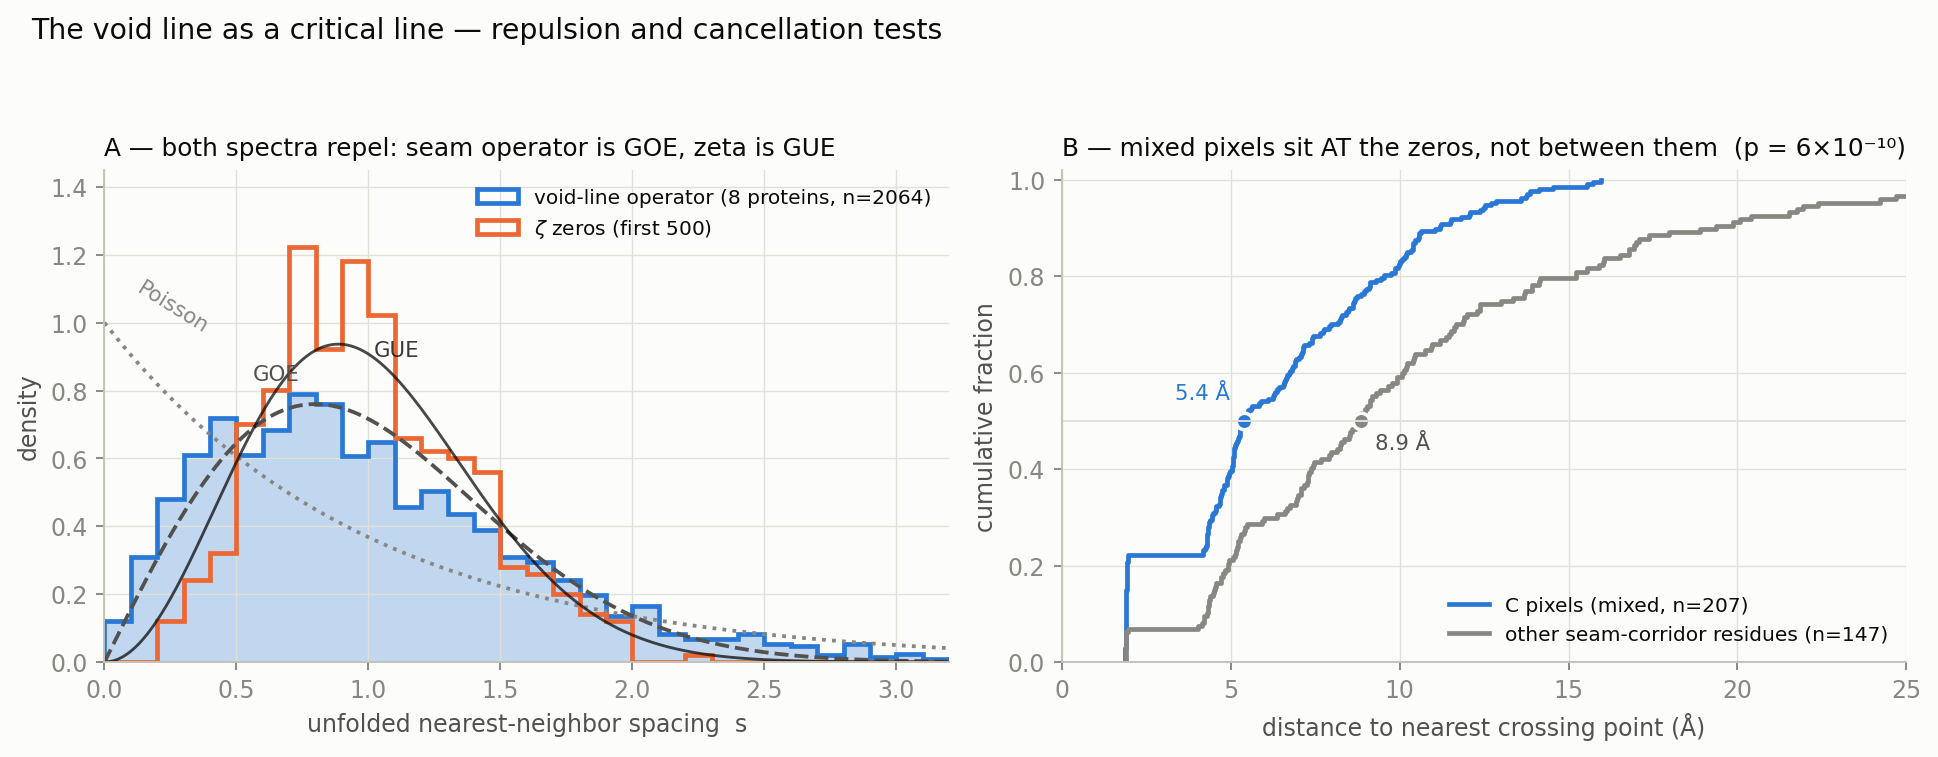
\includegraphics[width=\textwidth]{critical_line.png}
\caption{Left: pooled unfolded spacings of the void-line operator (blue, GOE) against the first 500
zeta zeros (orange, GUE), with the three reference laws. Right: the framework's mixed (cross-domain
contacting) residues concentrate at the seam-crossing points --- the zeros of the local signed field
--- rather than between them (median 3D distance 5.4\,\AA{} vs 8.9\,\AA{}, $p=6\times10^{-10}$).}
\label{fig:classes}
\end{figure}

\subsection{Mixed elements sit at the zeros}

The framework predicted its mixed (``C-pixel'') elements would occupy the non-zero stretches between
cancellation points. The measurement reversed the prediction: mixed residues concentrate \emph{at}
the crossings (median distance to nearest crossing 5.4\,\AA{} vs 8.9\,\AA{} for other corridor
residues; $p=6\times10^{-10}$; direction preserved under a centrality-matched control). The reversal
tightens the analogy: a zeta zero is not absence but exact cancellation of two present
contributions --- between zeros the Hardy function $Z(t)$ holds one sign (one side dominating), and
the zero is the only point where both sides are fully present and balanced. Mixture lives at the
zeros; dominance lives between them.

\subsection{The edge: de Bruijn--Newman flow}

RH is equivalent to $\Lambda\le0$ for the de Bruijn--Newman constant, and $\Lambda\ge0$ is a theorem
\cite{rodgerstao}; hence RH $\iff \Lambda=0$: the zero configuration sits exactly on the edge of the
heat flow, with no slack. Under the pair dynamics of the flow, isolated zero pairs collide at
$t=\mathrm{gap}^2/8$ (verified to five decimals); the tightest pair among the first 500 zeros
($\gamma\approx750.76$, gap $0.310$) collides at $t=0.0123$ against $\sim0.10$ for a typical pair,
and known closer (Lehmer) pairs above push the slack toward zero. In framework terms this is the
``ring at the maximum'': the unstoppable-force/unmovable-object standoff realized as a theorem-adjacent
fact.

\subsection{The golden field}

The corpus's orchard optimum lives in $\Q(\sqrt5)$ with closure discriminant 5. The corresponding
$L$-function is $L(s,\chi_5)$ with $\zeta_{\Q(\sqrt5)}=\zeta\cdot L(\cdot,\chi_5)$. Measurements:
$L(1,\chi_5)=2\ln\varphi/\sqrt5=0.430408940964$ verified to 15 digits (later identified as the class
number formula: the residue equals the shell volume, regulator $\ln\varphi$); 397 zeros of
$L(s,\chi_5)$ computed to $T=500$ against 396.8 predicted; the family is GUE-class; and the union
with the zeta zeros on the shared line loses repulsion exactly as an independent superposition
(alternation $z=-1.05$, small-spacing $z=-1.56$ against a 200-shift null): the two truth families
share the axis but are statistically blind to each other (Fig.~\ref{fig:rhlabs}).

\begin{figure}[t]
\centering
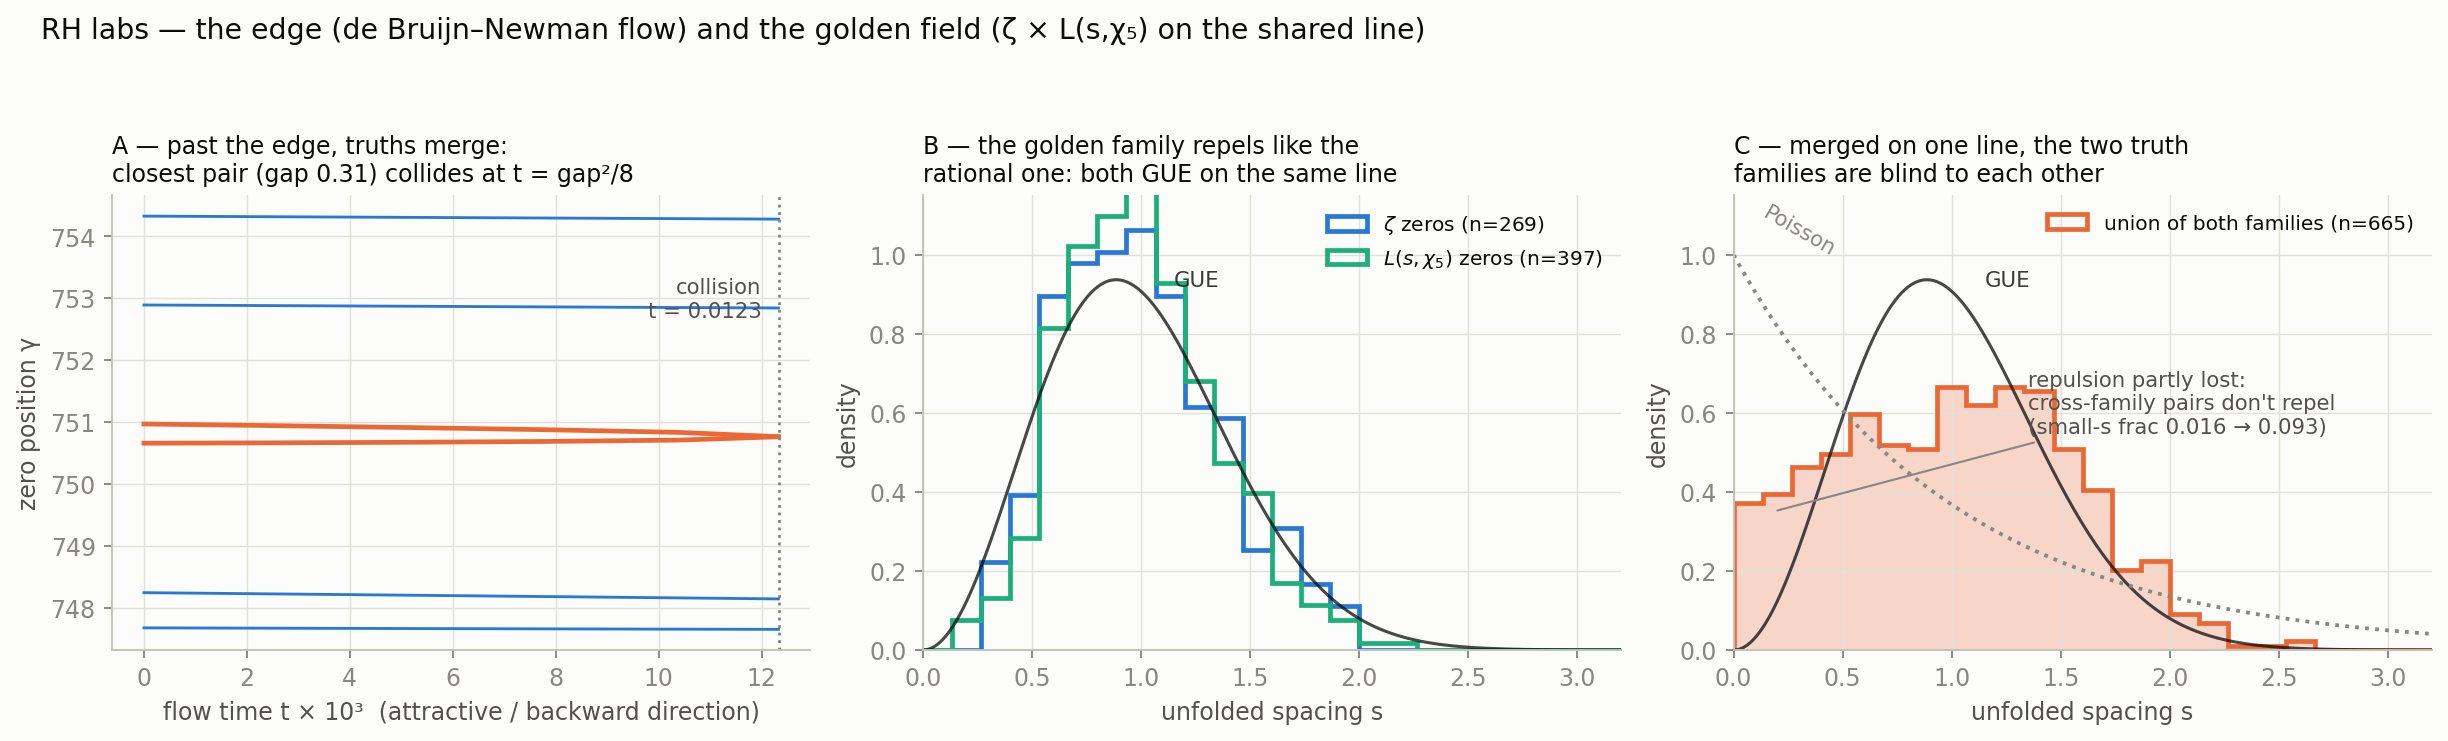
\includegraphics[width=\textwidth]{rh_labs.png}
\caption{Left: backward heat flow collapsing the tightest zero pair (the de Bruijn--Newman edge).
Centre: the $\chi_5$ family repels like the rational family (both GUE). Right: merged on one line,
the families' union loses repulsion --- consistent with independent superposition.}
\label{fig:rhlabs}
\end{figure}

\subsection{Berry--Keating: the clock's gears are the primes}\label{sec:bk}

Three measurements on the first 500 zeros. The $xp$ phase-space count
$N(E)=\frac{E}{2\pi}(\ln\frac{E}{2\pi}-1)+\frac78$ matches the true zero indices with mean residual
$-3\times10^{-5}$. The Fourier transform of the zero fluctuations shows towers $30$--$47\times$
background at exactly $u=k\ln p$ (including prime powers with the $p^{-k/2}$ fade): the truths ring
at the primes' orbit periods. Running it forward, 344 prime orbits rebuild the zero positions
(correlation 0.87; mean peak offset 0.019 of the mean spacing) --- the explicit formula as a trace
formula, measured (Fig.~\ref{fig:bk}).

\begin{figure}[t]
\centering
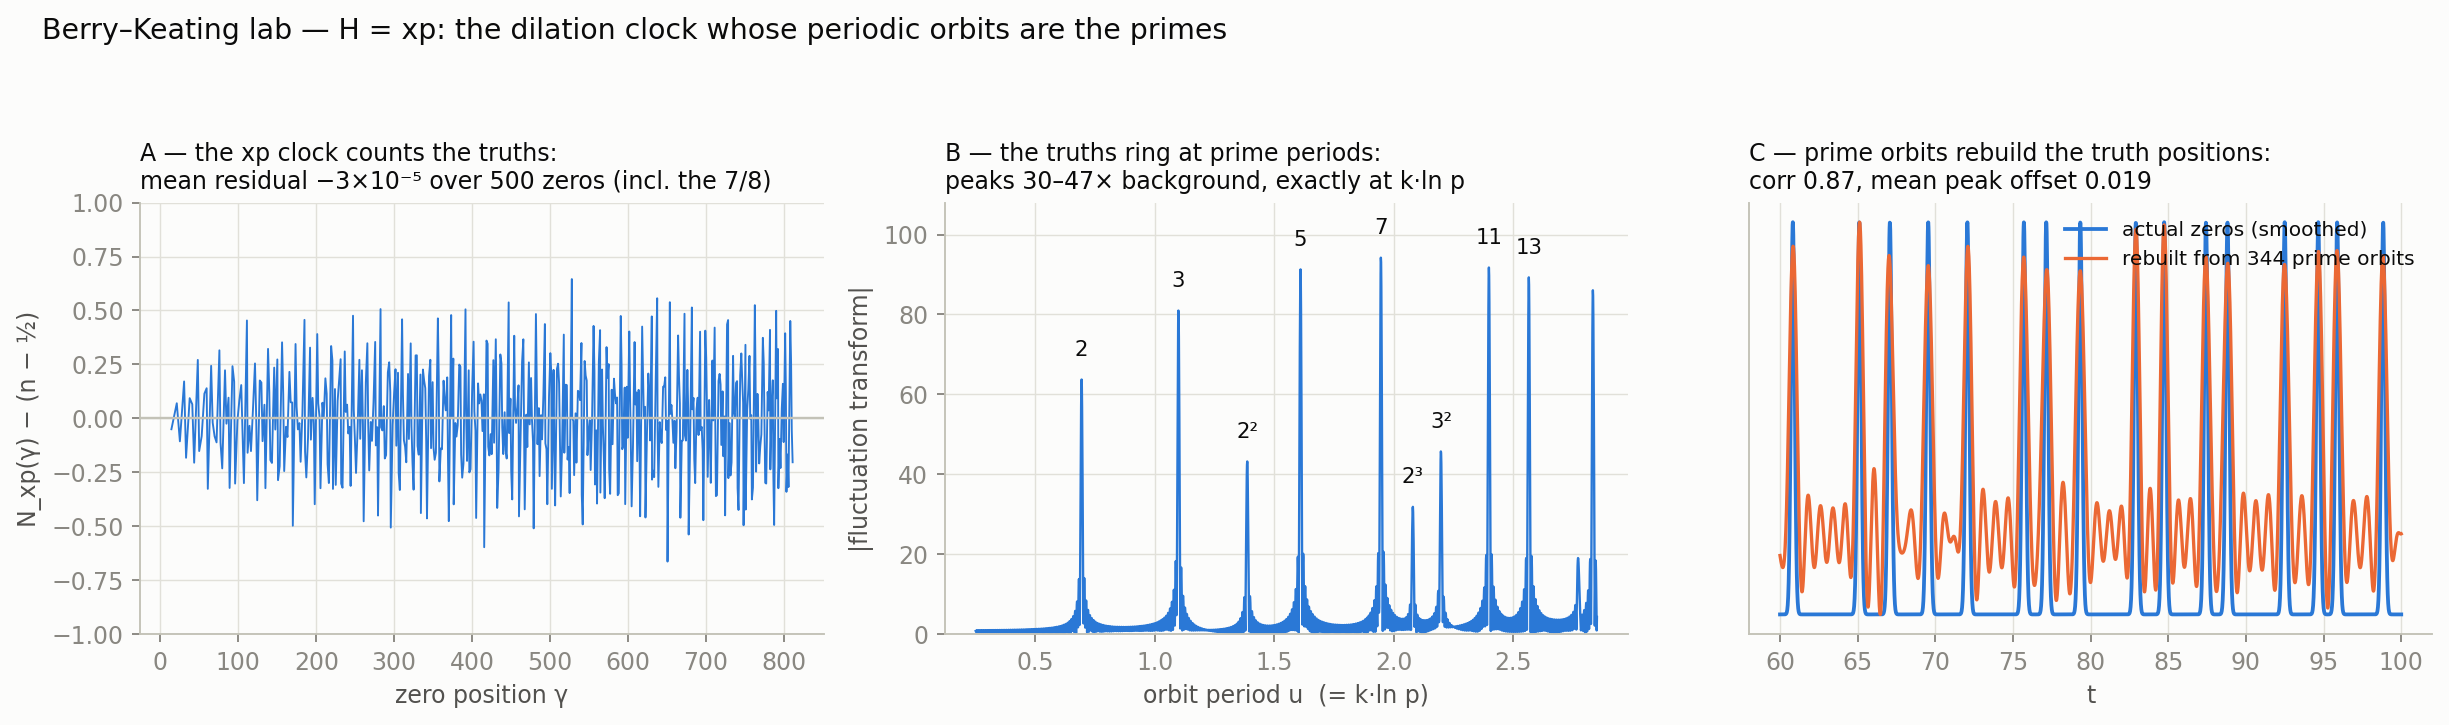
\includegraphics[width=\textwidth]{bk_lab.png}
\caption{The $xp$ clock: the semiclassical count (left), the prime-period resonances of the zero
fluctuations (centre), and the reconstruction of zero positions from prime orbits (right).}
\label{fig:bk}
\end{figure}

\section{The expander flip and the structure meter}\label{sec:expander}

\subsection{The folding plane fails its own RH}

Every finite graph carries an Ihara zeta function whose ``RH'' (Ramanujan condition) confines the
non-backtracking (Hashimoto) spectrum's non-trivial eigenvalues to the critical circle
$|\lambda|=\sqrt\rho$ --- proven territory on this plane. The eight protein contact graphs fail it,
0/8, and fail \emph{harder than chance}: the adjacency test gives $\lambda_2\approx9.4$--$11.8$
against Ramanujan bounds $5.5$--$6.2$, and the off-circle deviation of the Hashimoto spectrum exceeds
degree-matched configuration-model nulls at $z=19$--$74$ in all eight. The off-circle mass is
structural: the real eigenvalues escaping the circle are, in the spectral-redemption reading
\cite{krzakala}, precisely the community (two-domain) structure --- the very Fiedler direction the
framework uses to \emph{find} the void line (Fig.~\ref{fig:ihara}).

This inverts into the sharpest framework statement of RH produced by the program:
\begin{obs}
A Ramanujan graph is a perfect expander: maximally mixed, no preferred cut, nothing to find. A
foldable structure earns its readability by violating graph-RH by a measured amount. RH is then the
statement that \emph{the integers have no seam}: square-root cancellation everywhere, no outlier
past the critical circle, nothing sectionable. The void-line toolkit detects seams; RH says the
number line has none to detect.
\end{obs}

\begin{figure}[t]
\centering
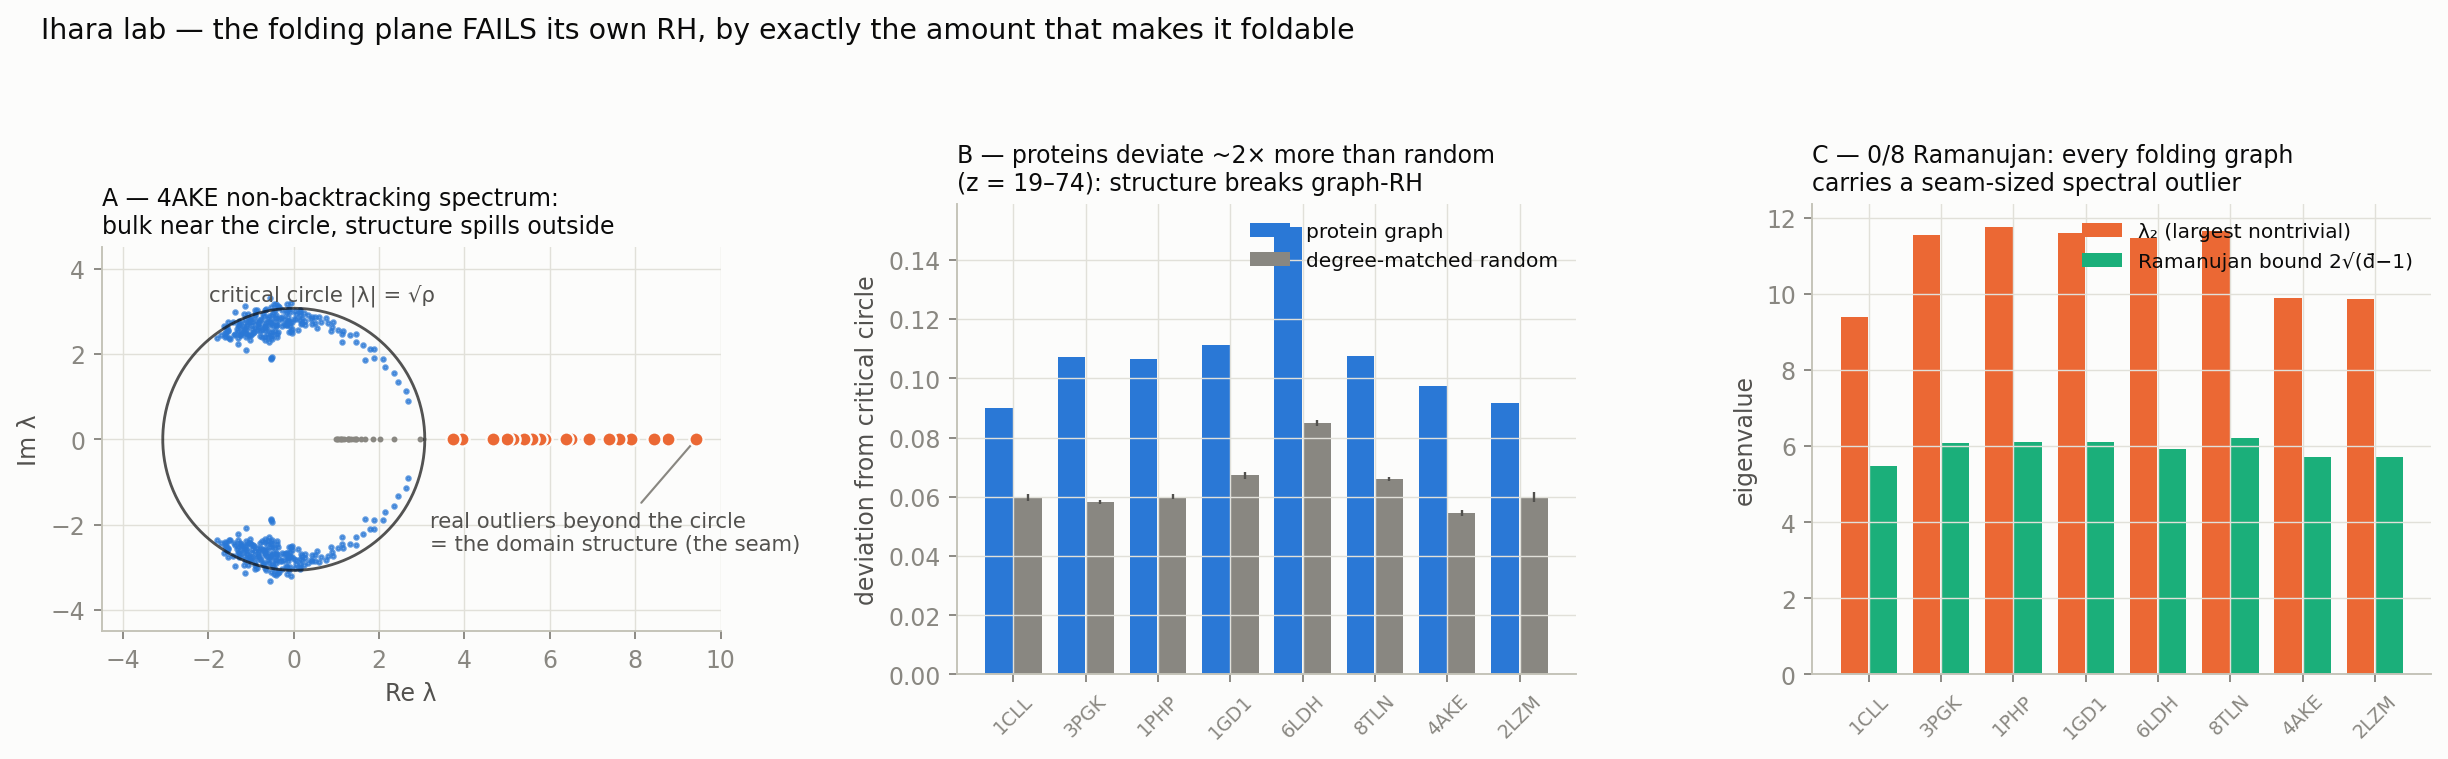
\includegraphics[width=\textwidth]{ihara_lab.png}
\caption{Left: the Hashimoto spectrum of 4AKE --- bulk near the critical circle, real outliers
(the domain structure) escaping it. Centre: proteins deviate about twice as far from their critical
circle as degree-matched random graphs. Right: 0/8 Ramanujan.}
\label{fig:ihara}
\end{figure}

\subsection{A cross-domain law and a solver signal}

Treating Ramanujan excess $\lambda_2/2\sqrt{\bar d-1}$ as a ``distance from RH,'' the program
measured it against seam strength ($-\log$ minimum sweep-cut conductance) across 299 graphs in six
domains: proteins, ARC task grids and their color-shuffled controls, Erd\H{o}s--R\'enyi graphs,
random 4-regular graphs, and lattice patches. The law holds at $r=0.527$, $p=8\times10^{-23}$
(Spearman), with the random-regular baseline landing on the Ramanujan line at excess $0.99$ and the
proteins at the far pole on both axes (Fig.~\ref{fig:meter}). On the ARC side, a region-compression
variant of the meter separates tasks solved by the corpus's ARC solver from unsolved tasks
(medians 1.38 vs 1.83, Mann--Whitney $p=0.017$, $n=93/307$) --- a modest but real routing signal,
delivered to the solver as the \texttt{structure\_meter} module. The cell-level encoding failed its
shuffle control (real $\approx$ shuffled) and was discarded; the region-adjacency encoding passes it
($p=9\times10^{-4}$), with the meter's sign depending on the reading plane --- the invariant is
displacement from the plane's own random baseline.

\begin{figure}[t]
\centering
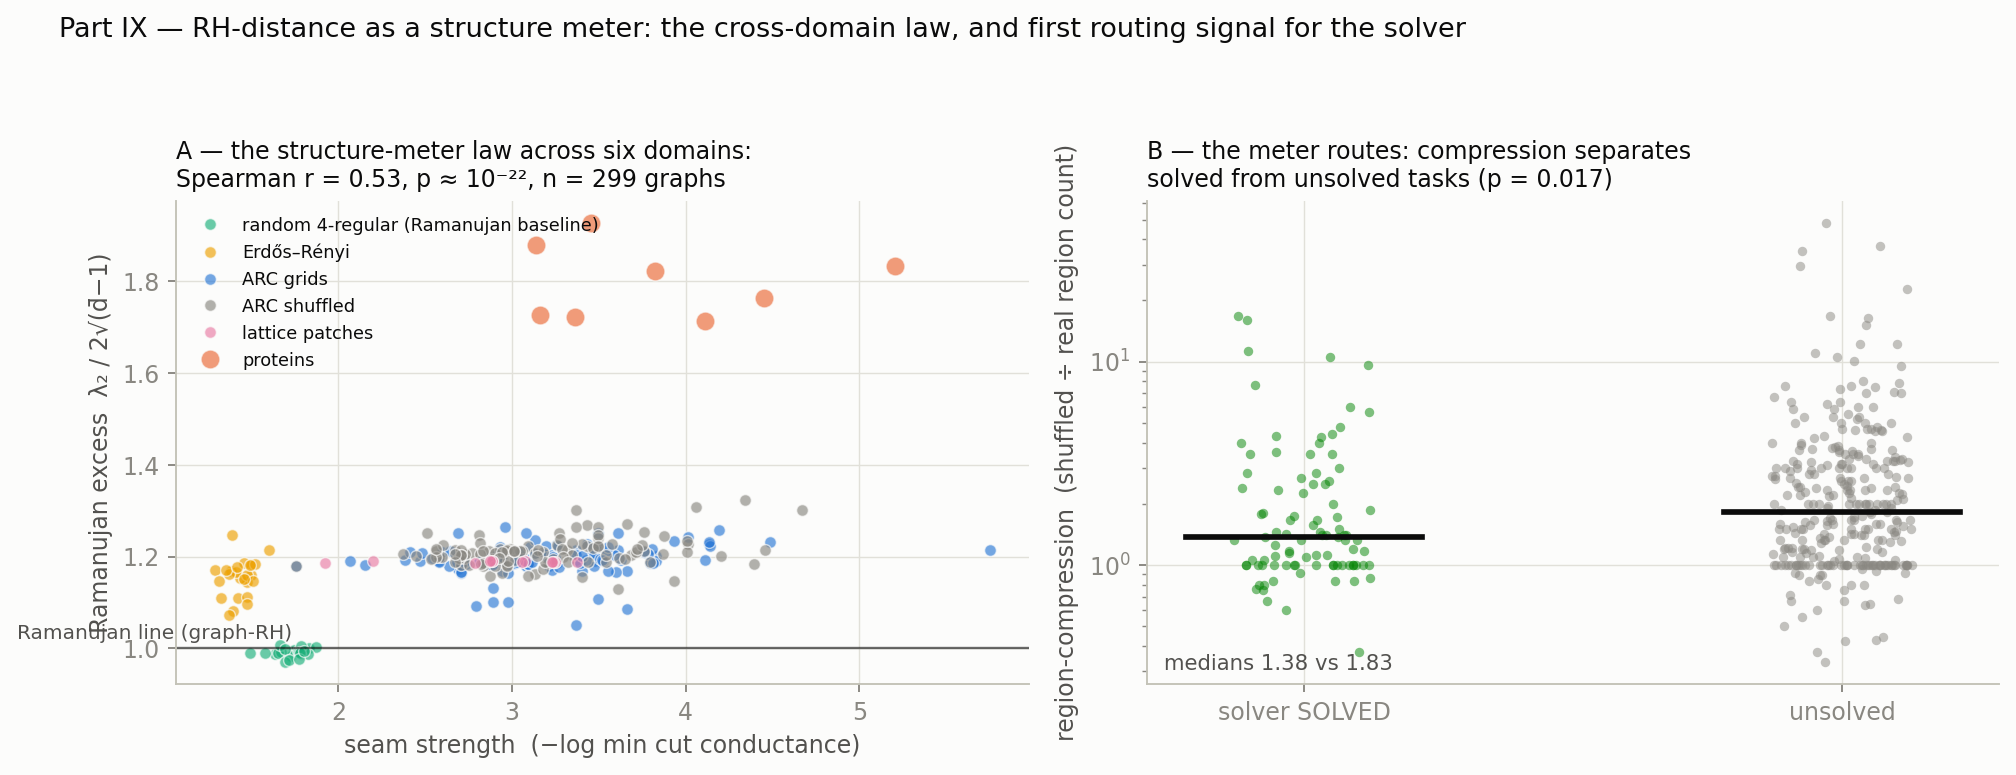
\includegraphics[width=\textwidth]{meter_law.png}
\caption{Left: seam strength vs Ramanujan excess over six domains; the random 4-regular baseline
sits on the Ramanujan line. Right: the region-compression meter separates solver-solved from
unsolved ARC tasks.}
\label{fig:meter}
\end{figure}

\section{Criterion laboratories}\label{sec:criteria}

\subsection{Nyman--Beurling: filling the void}

RH is equivalent to the constant function $1$ lying in the $L^2(0,1)$ closure of the dilated
fractional parts $\{1/(kx)\}$ \cite{bbls}. Measured: the unfilled distance obeys
$d_N^2\,\ln N\to C$ with the measured values $0.045$--$0.048$ against the conjectured
$C=2+\gamma-\ln4\pi\approx0.0462$ --- a constant that is $\sum_\rho|\rho|^{-2}$, the void points'
inverse-square masses as the filling resistance. The optimal filling coefficients track the
M\"obius function ($r=-0.92$, signs perfectly inverted): the void is filled by inclusion--exclusion,
the framework's $+/-$ alternation (Fig.~\ref{fig:nbli}, left).

\subsection{Li's ledger and the counterfeit alarm}

RH is equivalent to the non-negativity of all Li coefficients $\lambda_n$ \cite{li}. From the 500
zeros with smooth tail correction: $\lambda_1=0.0231$ (the known exact value to four decimals), all
positive through $n=80$. Injecting one off-line quadruple at $0.75\pm2i$ flips the ledger negative
at $n=64$ (minimum $-105$): positivity is a working alarm whose ring period and envelope encode the
counterfeit's position (Fig.~\ref{fig:nbli}, right).

\begin{figure}[t]
\centering
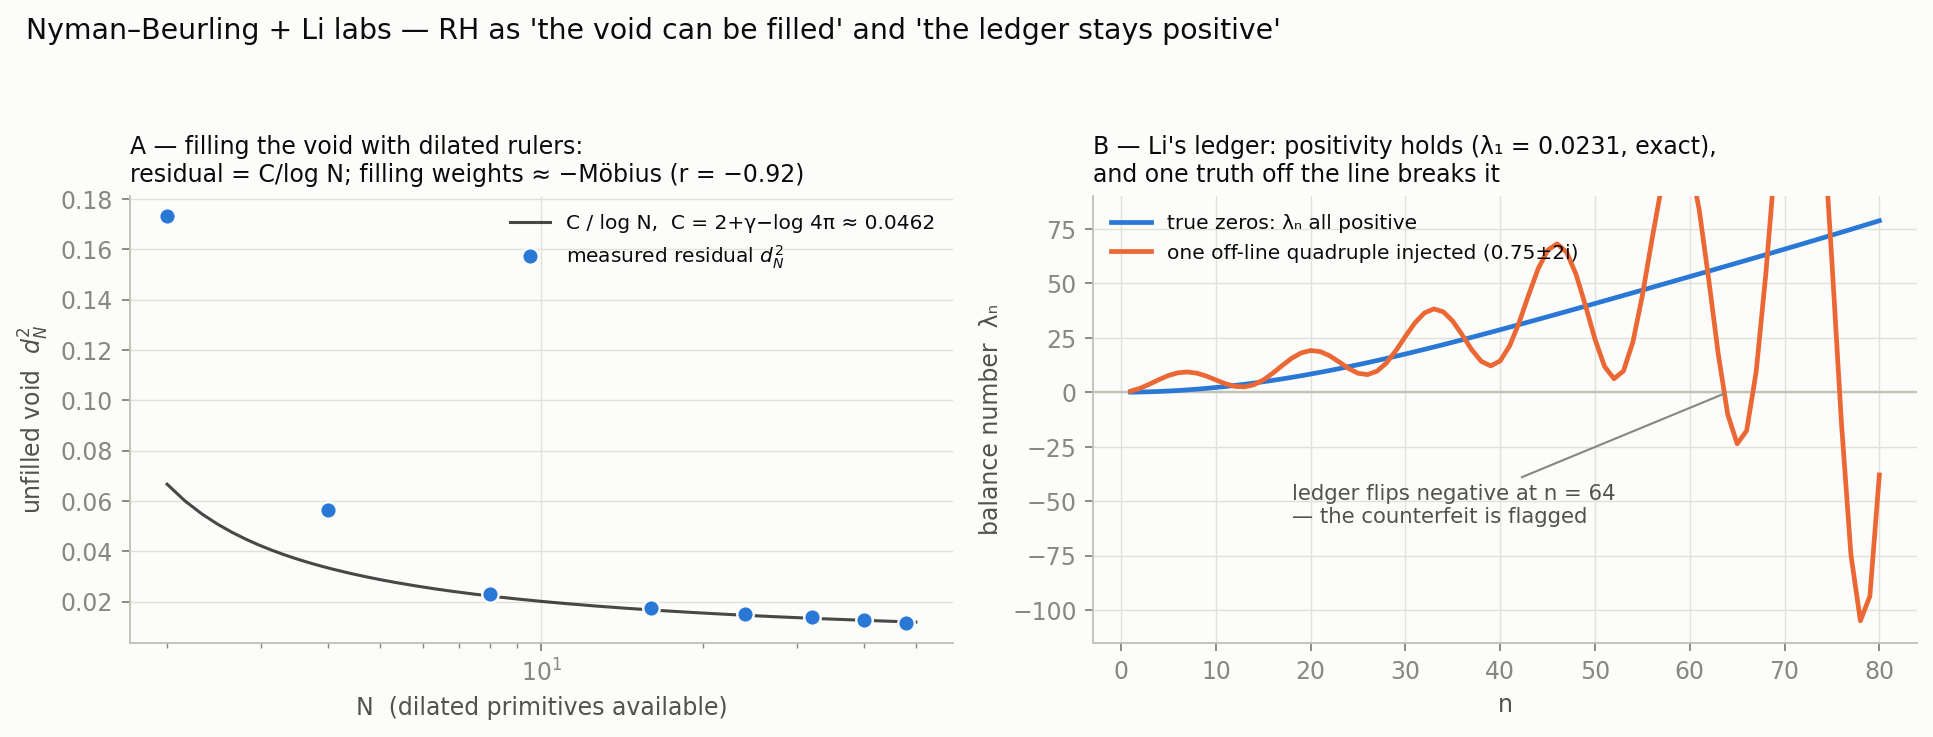
\includegraphics[width=\textwidth]{nb_li.png}
\caption{Left: the Nyman--Beurling fill law $d^2_N=C/\ln N$ with $C=2+\gamma-\ln4\pi$. Right: Li's
$\lambda_n$, all positive for the true zeros; one off-line quadruple bankrupts the ledger at
$n=64$.}
\label{fig:nbli}
\end{figure}

\section{Thermodynamic identifications}\label{sec:thermo}

The primon gas \cite{julia} realizes the framework's thermodynamics exactly, and the program
verified its identities directly: the many-particle states of free bosons with mode energies
$\ln p$ \emph{are} the integers (unique factorization as occupation numbers), the partition function
is $\zeta(\beta)$ ($\zeta(2)=\pi^2/6$ checked to 12 digits), each gear's occupation is the
Bose--Einstein distribution $1/(p^\beta-1)$ (checked against a direct 200{,}000-state sum), and the
thermal energy is $-\zeta'/\zeta$ (checked against the prime-orbit sum). The pole is a
\emph{Hagedorn ceiling}: $S/E\to1$ exactly, so temperature cannot exceed $T=1$; heat pushed in near
the wall converts to new modes rather than warmth ($U:1.5\to199$ as $T:0.67\to0.995$). Below the
ceiling, the Bost--Connes system \cite{bostconnes} condenses with the symmetry broken being exactly
the observers' rotation group --- the framework's ``observer angles freezing.'' The minimal erasure
cost at the natural temperature, $k_BT\ln2$ with $k_BT=1$, coincides with the smallest gear's
orbit period $\ln 2$ --- Landauer's bound \cite{landauer} priced in the gas's own ground mode.
Finite stages close at $0.999\ldots$ (Mertens with $e^\gamma\ln P$ normalization: $0.9961$,
$0.99970$, $0.99996$ at 168, $9.6$k, $78$k gears); exact closure belongs to the completed limit.

\section{The field machine}\label{sec:machine}

\subsection{The smooth phase from the ray source}

The $\theta$-field equation of \cite{pelchat-theta},
$\partial_t\theta = D\nabla^2\theta-(\theta-1)/\tau+S$, was solved in its stationary, frictionless
($\tau\to\infty$) regime on the line, $\theta''=S/D$, for three candidate sources. A point source
(linear profile) misses the true Riemann--Siegel $\theta(t)$ by RMS 67.8; a uniform source
(quadratic) by 15.7; the \emph{ray source} $S\propto1/x$ --- the Haar measure $dx/x$ of the scaling
ray, the framework's canonical ``immovable pile'' --- lands at RMS $9\times10^{-5}$. The two
integration constants, fitted freely, return $-0.9189387$ and $-0.3925$, i.e.\
$-\tfrac12\ln2\pi$ (seven figures) and $-\pi/8$ (the source of the $7/8$ in the counting formula).
With both constants \emph{fixed} at these $\pi$-values, the residual equals the known $1/(48t)$
asymptotic tail of $\theta$ to nine significant figures at every checkpoint. With the relaxation
term restored ($\tau=100$) the profile is screened to $10^{-5}$ of the truth: the mechanism requires
precisely the frictionless regime the corpus independently assigns to the void line
(Fig.~\ref{fig:bridge}).

\begin{figure}[t]
\centering
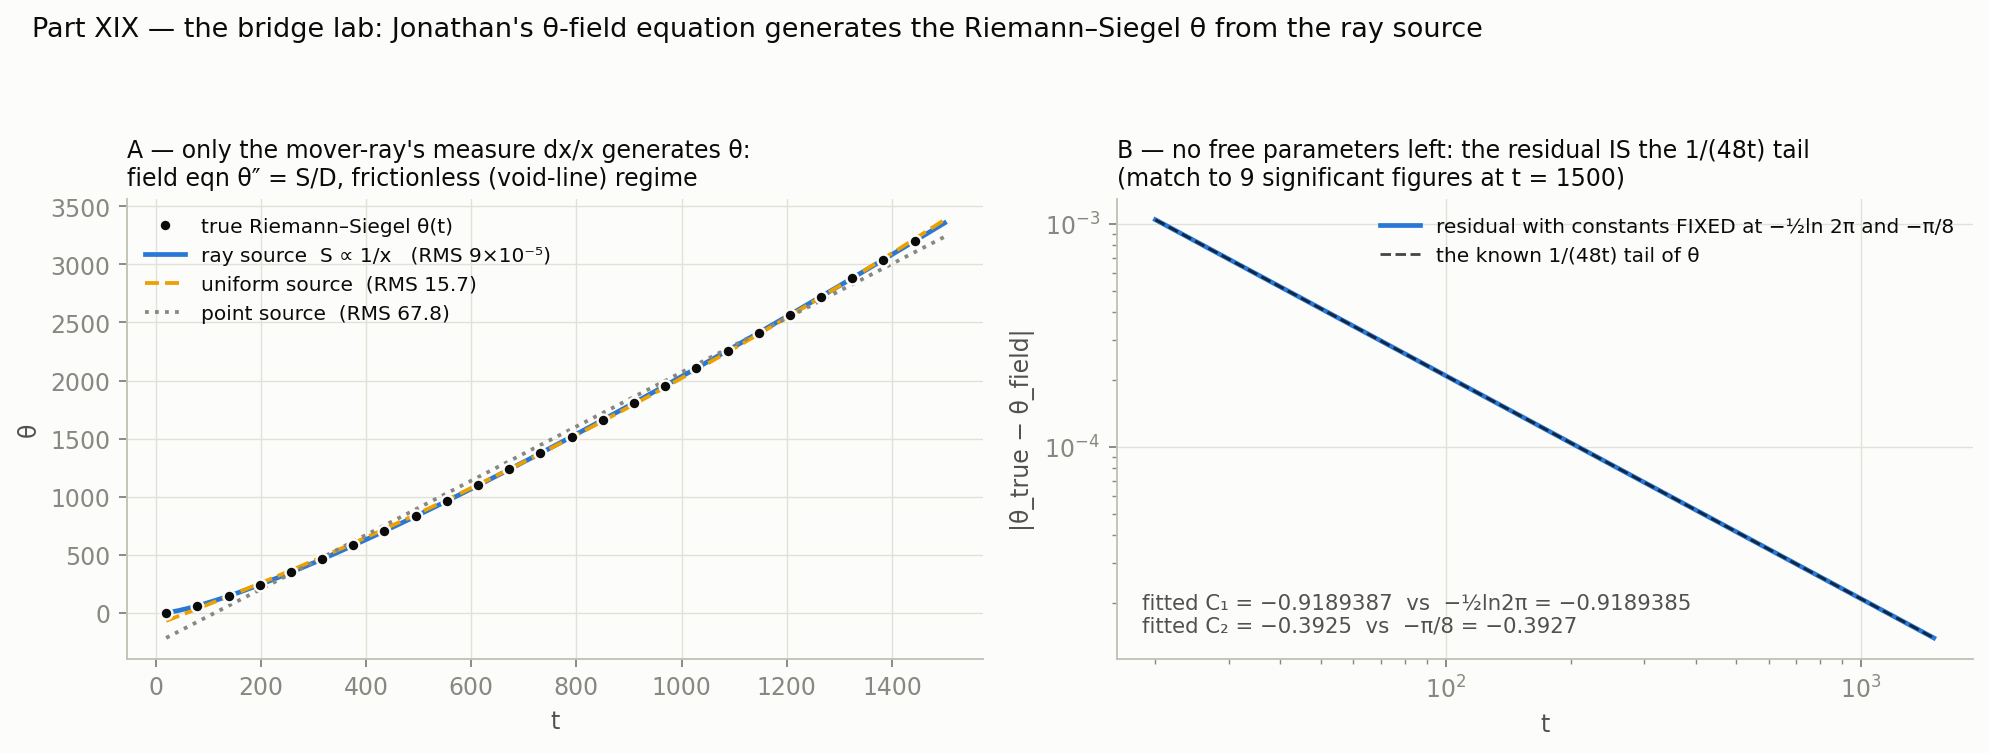
\includegraphics[width=\textwidth]{theta_bridge.png}
\caption{The bridge laboratory. Left: only the ray source generates $\theta$. Right: with the
integration constants fixed at $-\tfrac12\ln2\pi$ and $-\pi/8$, the residual collapses onto the
known $1/(48t)$ tail.}
\label{fig:bridge}
\end{figure}

\subsection{The fluctuation from the gear sources}

Adding to the same equation the gear sources --- oscillatory terms at the wall-ladder frequencies
$k\ln p$ with weights $p^{-k/2}$ --- generates the fluctuation
$S(t)=N(t)-\theta(t)/\pi-1$: correlation with the true sawtooth rises $0.46\to0.70\to0.84\to0.90$
at $1, 4, 25, 168$ gears (RMS $0.33\to0.16$ against a signal s.d.\ of $0.37$), the residual living
in the sharp corners at the jumps --- the usual logarithmic tail (Fig.~\ref{fig:gears}). The full
phase $\pi N(t)=\theta(t)+\pi S(t)+\pi$ is thereby generated by one field equation from two
framework-named sources. Stated honestly: this is the explicit formula recast as a field mechanism,
taking the primes as given; its value is that both halves now run inside the published field law
with no free constants.

\begin{figure}[t]
\centering
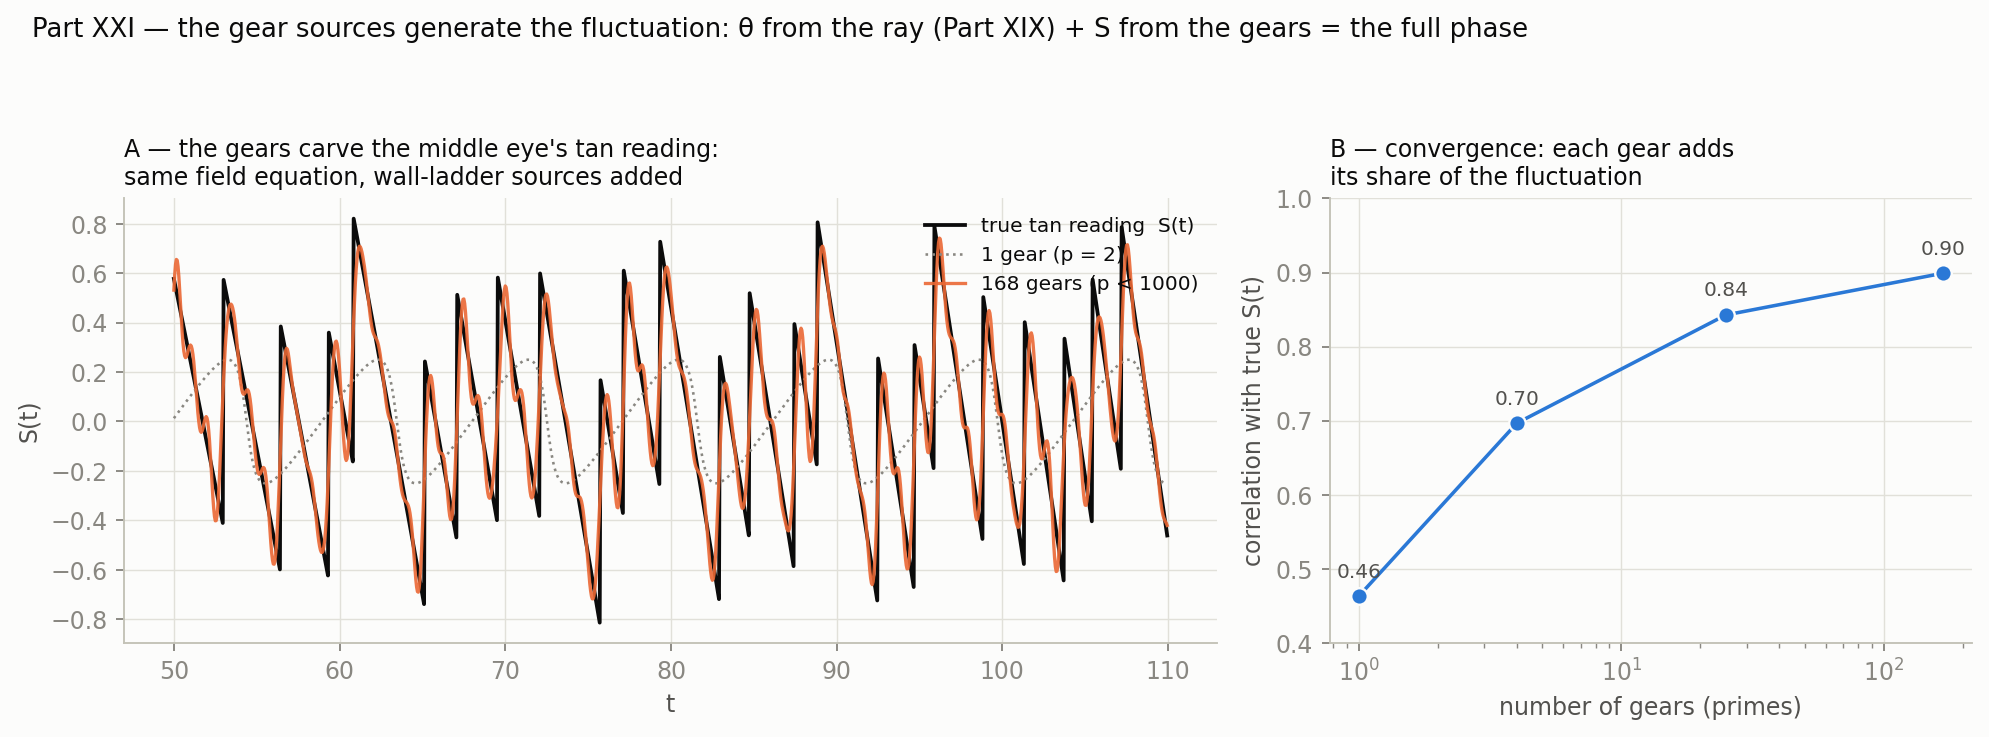
\includegraphics[width=\textwidth]{gear_lab.png}
\caption{The gear laboratory: the same field equation with wall-ladder sources carves the true
fluctuation $S(t)$; convergence with gear count at right.}
\label{fig:gears}
\end{figure}

\subsection{The weave}

Figure~\ref{fig:weave} shows the critical strip face-on: the zero sets of $\mathrm{Re}\,\zeta$ and
$\mathrm{Im}\,\zeta$ fill it as a woven sheet (the classical ``X-ray''). The $\mathrm{Re}$-threads
hairpin exactly at the zeros, pinned to the midline; the $\mathrm{Im}$-threads run out to touch
both walls and cross the midline at the Gram points --- the slots. Truths and slots alternate as
the two families take turns touching the waist. The trigonometric decomposition matches the
framework's assignment: the wall sweeps are cosine threads ($Z=2\sum\cos(\theta-t\ln n)/\sqrt n$),
the reflection factor carries the sine ($\chi(s)=2^s\pi^{s-1}\sin(\pi s/2)\Gamma(1-s)$, whose zeros
are the trivial ladder --- the fold behind the $0$ wall), and the central reading is the tangent:
$S(t)=\frac1\pi\arg\zeta(\tfrac12+it)$, the ratio of the two thread families. In this vocabulary RH
reads: \emph{every hairpin turns exactly on the waist}.

\begin{figure}[t]
\centering
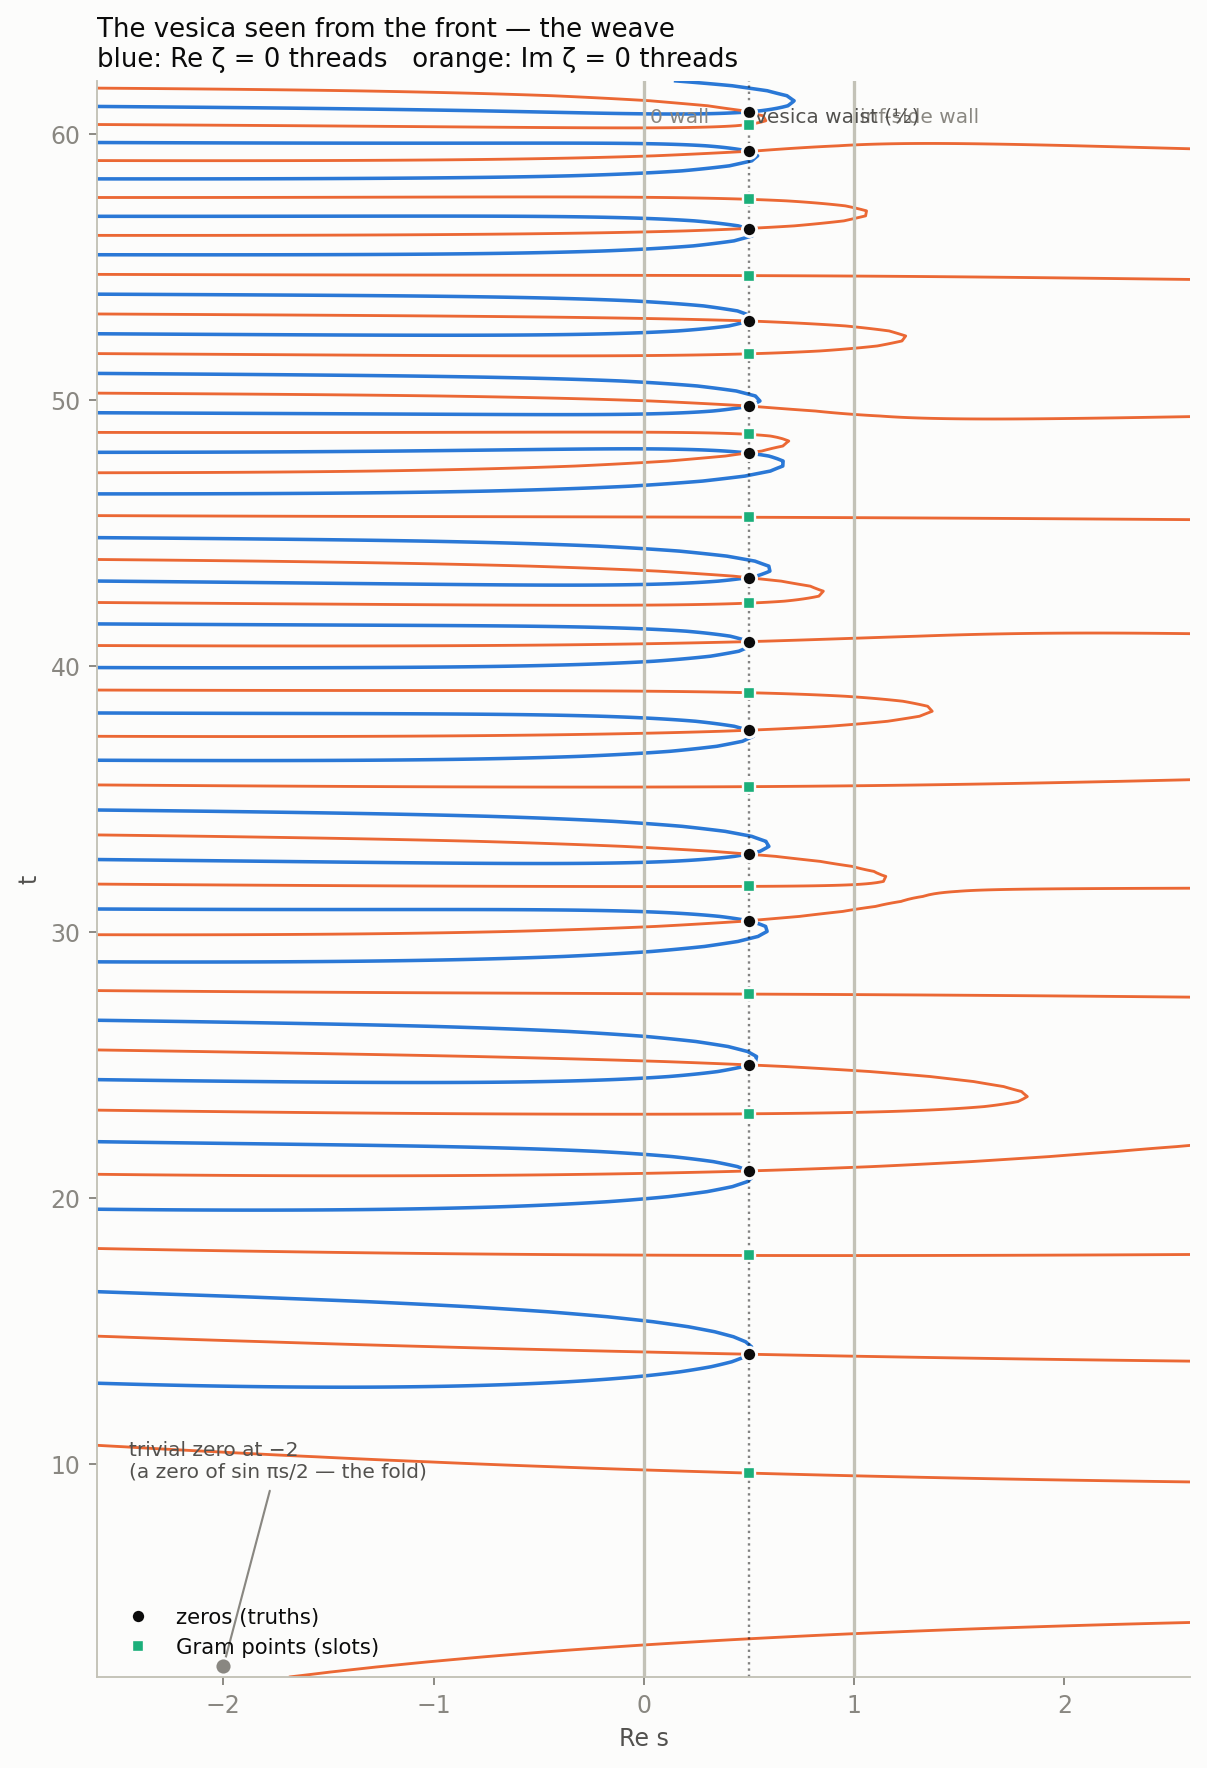
\includegraphics[width=0.62\textwidth]{vesica_weave.png}
\caption{The strip face-on: $\mathrm{Re}\,\zeta=0$ threads (blue) hairpinning at the zeros;
$\mathrm{Im}\,\zeta=0$ threads (orange) anchoring to the walls and crossing the waist at Gram
points; the trivial zero at $-2$ flat behind the left wall.}
\label{fig:weave}
\end{figure}

\section{The correspondence table}\label{sec:table}

Table~\ref{tab:corr} collects the mapping assembled by the program. Entries marked (M) are
in-session measurements; (T) are identifications with named theorems or standard objects.

\begin{table}[t]
\centering\small
\begin{tabular}{@{}lll@{}}
\toprule
Framework object & Mathematical object & Status\\
\midrule
void line & critical line $\mathrm{Re}\,s=\tfrac12$ & program thesis\\
void points / truths & non-trivial zeros & (M) spacings, (T) explicit formula\\
slots / available positions & Gram points and intervals & (T)\\
slot borders / sign stretches & sign changes of Hardy $Z$ & (T)\\
mixed pixels & cancellation at the zeros & (M) $p=6\times10^{-10}$\\
re-based recursive void & Dirichlet $L$-functions, GRH & (T)\\
golden field shell & $\Q(\sqrt5)$: $\zeta_K=\zeta\cdot L(\cdot,\chi_5)$, disc.\ 5 & (T,M)\\
observers (enclosed, rotating, cone) & places of $\Q$; $\Z_p$, units $\Z_p^\times$, $|\cdot|_p$ & (T)\\
observer shell & unit sphere; Gauss sum, $|\tau|=\sqrt q$ & (T,M)\\
internal rotation $\times$ mover & idele class group $=$ compact $\times\,\R_+$ & (T)\\
the mover / tick source & pole at $s=1$, residue exactly 1 & (T,M)\\
shave $\varepsilon$, weight $1/\varepsilon$, leftover & $\zeta(1+\varepsilon)=1/\varepsilon+\gamma$ & (M)\\
mover's push $=$ shell size & class number formula & (T,M)\\
clock gears & primes as periodic orbits, periods $\ln p$ & (M) 30--47$\times$ resonances\\
gear trails on the $0$ wall & zeros of $1-p^{-s}$ at $2\pi ik/\ln p$ & (M) $10^{-15}$\\
no-resonance / golden constraint & $\ln p/\ln q$ irrational (unique factorization) & (T)\\
fold behind the $0$ base & trivial zeros; $\zeta(0)=-\tfrac12$, $\zeta(-1)=-\tfrac1{12}$ & (T,M)\\
flattening energy banked in the fold & $\Gamma$-poles cancel trivial zeros ($\xi(-2)\ne0$) & (M)\\
transfer law across planes & product formula $\prod_v|x|_v=1$ & (T,M)\\
quaternion closure check & Hilbert reciprocity $\prod_v(a,b)_v=1$ & (T)\\
$.999\ldots$ working closure & Mertens partial products & (M)\\
BEC / condensate in the eye & primon gas, Bost--Connes phase transition & (T,M)\\
Hagedorn plasma / frozen centre & maximum temperature $T=1$ at the pole & (M)\\
Landauer burn of the shaved piece & $k_BT\ln2$ $=$ ground gear period & (M)\\
walls curving to face each other & completion factor $\pi^{-s/2}\Gamma(s/2)$ & (T)\\
heat flattening the ring & Jacobi $\theta$; Poisson summation; $\theta(1/x)=\sqrt x\,\theta(x)$ & (M) 12 digits\\
the $\tfrac12$ as base-shift exponent & the $\sqrt x$ in the theta transformation & (T)\\
overlap shave at the wall & boundary terms $-1/s-1/(1-s)$ in Riemann's proof & (M)\\
pupil, one cell, rim $7/8$ & excised $2\pi$ phase-space cell; Maslov-type constant & (T,M)\\
central eye at the midpoint & Riemann--Siegel formula; cutoff $\sqrt{t/2\pi}$ & (M)\\
central eye's rotation at handoff & $\chi(\tfrac12+it)=e^{-2i\theta(t)}$ & (T)\\
side-lines' central readings & central values $L(\tfrac12,\chi)$; Katz--Sarnak families & (T)\\
vesica lens / equator & critical strip / critical line & (T)\\
load field $\theta(r,t)$ & Riemann--Siegel $\theta(t)$ via the field equation & (M) \S\ref{sec:machine}\\
distance-from-RH as structure meter & Ramanujan excess; seam law $r=0.53$ & (M)\\
\bottomrule
\end{tabular}
\caption{The correspondence assembled by the program. (M) $=$ measured in-session;
(T) $=$ identification with a named theorem or standard object.}
\label{tab:corr}
\end{table}

\section{Discussion: what is established, and the one remaining door}\label{sec:discussion}

What the program establishes is a systematic, quantitative correspondence: the framework's
primitives map onto named objects of analytic number theory, in most cases exactly, and the
framework's own field law generates the complete phase of $\zeta$ from two of its named sources with
all constants forced. Where framework predictions failed (mixed pixels between the zeros; the
cell-plane structure meter), the failures were caught by designed controls and the corrections
tightened the mapping. The cross-domain seam law of \S\ref{sec:expander} appears to be new as a
measurement, as does the framing of the routing signal for the ARC solver.

What the program does not touch is RH itself, and the assembled machine makes the remaining
question precise. The explicit-formula mechanism of \S\ref{sec:machine} takes the primes as given
and reconstructs the zeros' phase; the open problem is the \emph{alignment law}: why the output of
the meshed gears always turns exactly on the waist --- equivalently, the self-adjoint completion of
the $xp$ clock whose closed orbits have periods $\ln p$ with weights $p^{-k/2}$ (the boundary
condition at the pupil, whose scattering phase must equal $\theta(t)$); equivalently $\Lambda=0$
with zero slack; equivalently the positivity of every $\lambda_n$; equivalently perfect expansion of
the integers. Every constraint on that missing mechanism measured here --- the magnitudes of the
shell integrals pinned at $\sqrt q$, the sign skeleton closed by reciprocity, the two views
coinciding only at the half, the Hagedorn ceiling at the pole --- is consistent with the framework's
central intuition that the line survives at its maximum, barely, with the slack exactly spent. The
framework's candidate contribution, should the program continue, is a closure-unit construction for
the phases of the shell integrals; the present paper is the specification of everything such a
construction must reproduce.

\section{Addendum (v2): the weave, the completed machine, and the pinning laboratory}

Six further laboratories were run after the first version of this paper.

\textbf{The weave.} The zero sets of $\mathrm{Re}\,\zeta$ and $\mathrm{Im}\,\zeta$ fill the strip as
two conjugate thread families (harmonic conjugates: each family's level curves are the other's flow
lines). The $\mathrm{Re}$-threads hairpin exactly at the zeros, pinned to the midline; the
$\mathrm{Im}$-threads run out to both walls and cross the midline at the Gram points --- truths and
slots alternating as the two families take turns touching the waist (Fig.~\ref{fig:weave2}). The
trigonometric decomposition is exact: cosine threads from the wall sweeps
($Z=2\sum\cos(\theta-t\ln n)/\sqrt n$), the sine in the reflection factor
$\chi(s)=2^s\pi^{s-1}\sin(\pi s/2)\Gamma(1-s)$ (whose zeros are the trivial ladder), and the central
tangent reading $S(t)=\frac1\pi\arg\zeta(\tfrac12+it)$.

\textbf{The machine completed.} Adding the gear sources (frequencies $k\ln p$, weights $p^{-k/2}$)
to the same field equation generates the fluctuation $S(t)$: correlation with the true sawtooth
$0.46\to0.70\to0.84\to0.90$ at $1,4,25,168$ gears (Fig.~\ref{fig:gears2}). With the ray source
producing $\theta$ (\S\ref{sec:machine}), the full phase $\pi N=\theta+\pi S+\pi$ is generated by
one field law from two framework-named sources.

\textbf{Vortex quantization.} The phase field $\arg\zeta$ winds by exactly $2\pi$ around every zero
(measured winding $1.000$ at the first and second zeros; $0.000$ at zero-free points): the
bidirectional flow's cancelled circulation condenses into one quantum per truth. RH in vortex form:
\emph{no circulation quantum ever drifts off the waist} --- a pinning statement, with vortex pinning
in condensates as the physical model.

\textbf{Outside the cones.} The visible structure is a measure-zero skeleton, and by Voronin's
universality theorem the off-line bulk approximates \emph{any} non-vanishing analytic function to
any accuracy, infinitely often: outside the committed skeleton is provably anything. On the proven
modular plane, the trace formula's continuous (Eisenstein) spectrum supplies the ``invisible gas'' ---
unbound states passing through the structure --- and its scattering phase is built from the completed
$\zeta$ itself.

\textbf{The pinning laboratory.} A first measured probe of the alignment law
(Fig.~\ref{fig:pinning}). The one-eyed approximant $\sum_{n\le N}n^{-s}$ (no mirror) scatters its
vortices across the strip (median $|\mathrm{Re}-\tfrac12|=0.270,\,0.128,\,0.028$ at $N=3,8,20$; none
on the line at small $N$). The two-eyed approximant
$\sum_{n\le N}n^{-s}+\chi(s)\sum_{n\le N}n^{s-1}$, which satisfies the exact functional equation,
pins \emph{every} vortex to the waist at grid resolution ($100\%$ on-line at $N=8$ and $20$). At
$N=3$ the only permitted escape is visible: two mirror \emph{pairs} off-line at symmetric positions
--- the pair channel --- and by $N=8$ the pairs are gone. The laboratory thus separates two pinning
forces (the mirror: fast; the meshing gears: slow) and localizes RH into a single sentence:
\emph{the completed function never uses the mirror-pair loophole}. Zeros of sections and symmetrized
sections are studied territory; the contribution here is the quantified two-force picture and the
localization.

\begin{figure}[t]
\centering
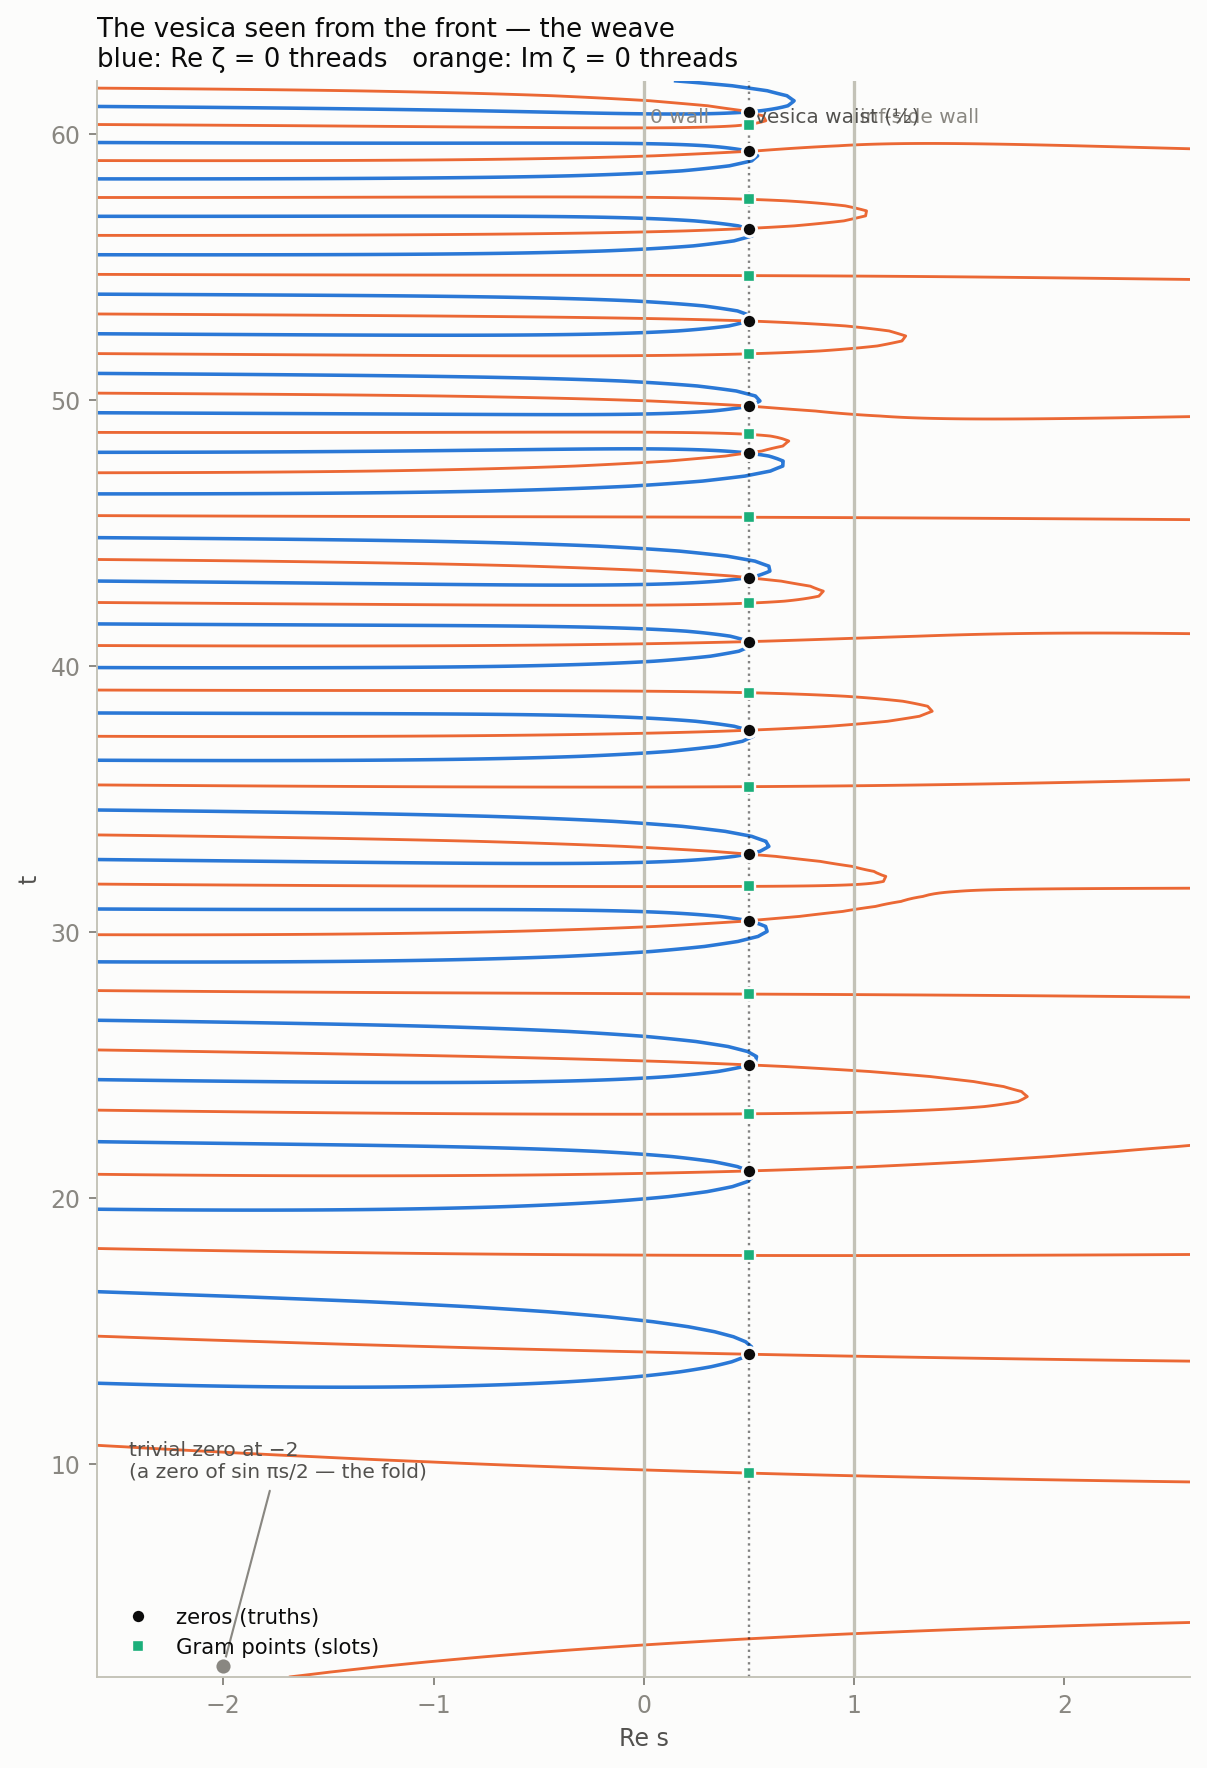
\includegraphics[width=0.5\textwidth]{vesica_weave.png}
\caption{The strip face-on: the conjugate thread families, truths at the blue hairpins, slots at the
orange wall-anchored crossings.}
\label{fig:weave2}
\end{figure}

\begin{figure}[t]
\centering
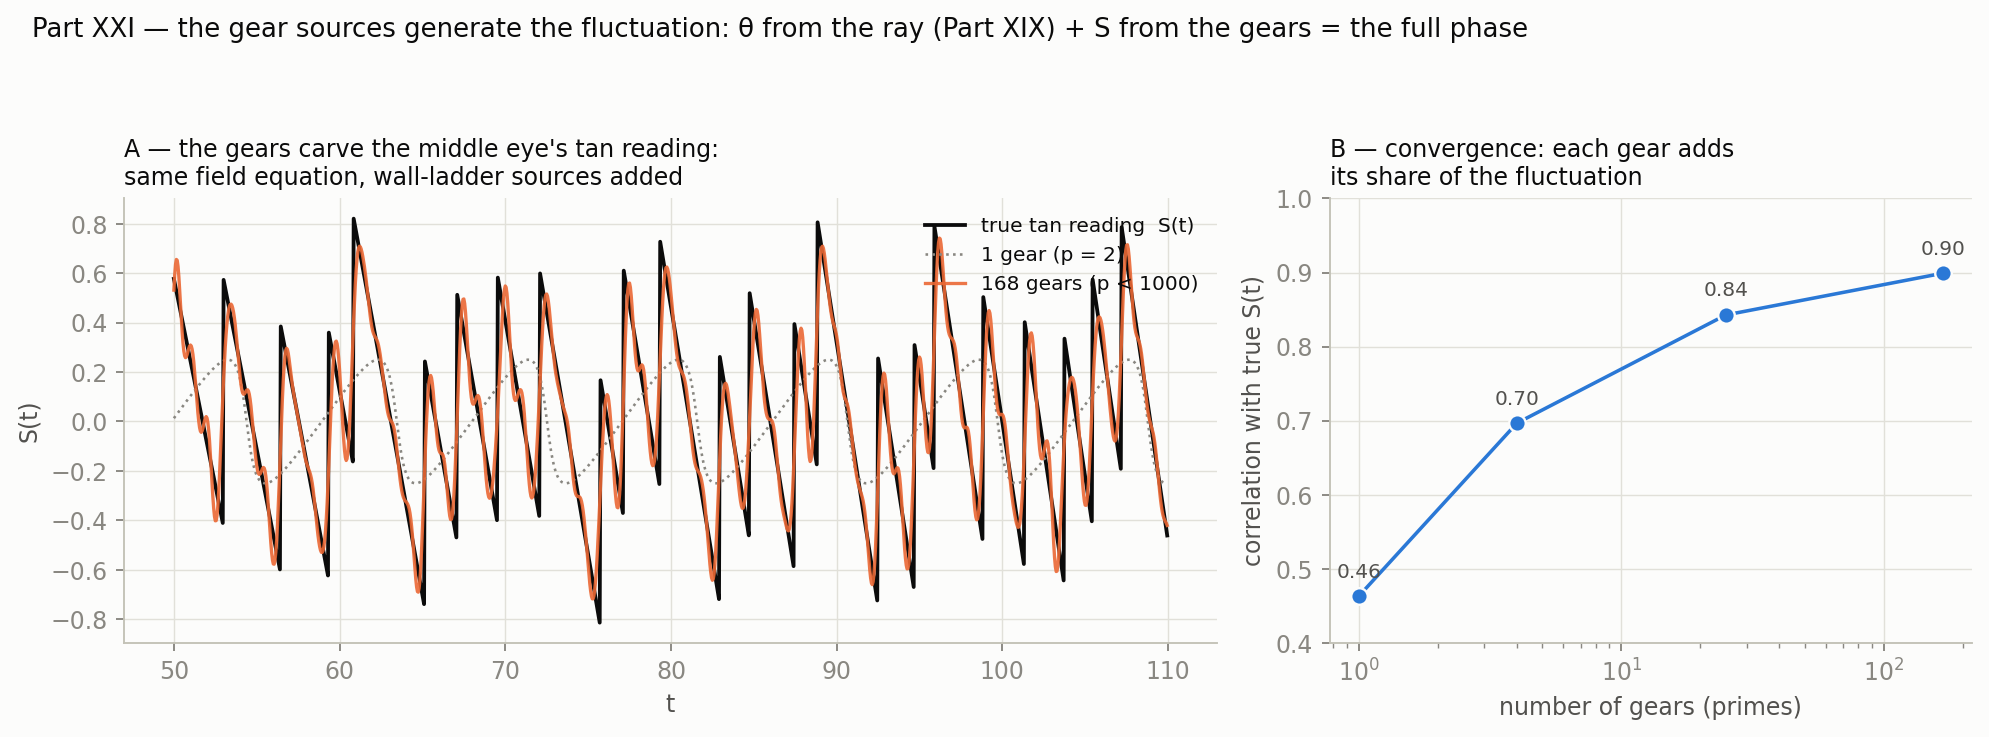
\includegraphics[width=\textwidth]{gear_lab.png}
\caption{The gear sources generate the fluctuation $S(t)$ in the same field equation that generates
$\theta$; convergence with gear count at right.}
\label{fig:gears2}
\end{figure}

\begin{figure}[t]
\centering
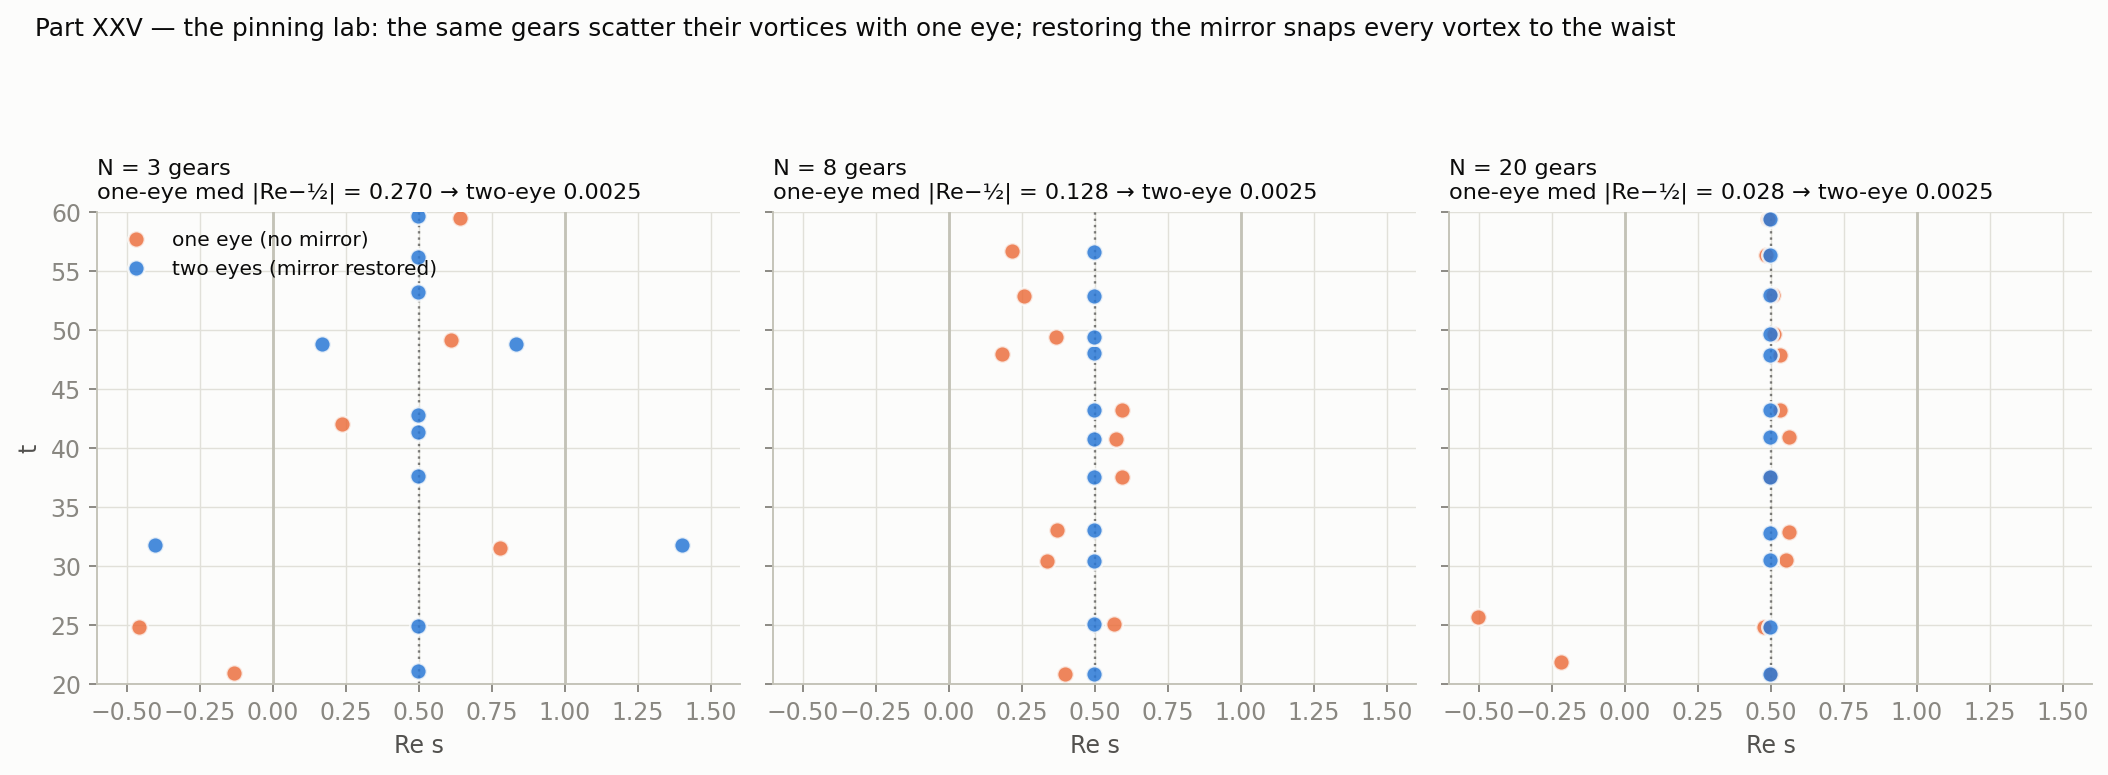
\includegraphics[width=\textwidth]{pinning_lab.png}
\caption{The pinning laboratory: one eye scatters, the restored mirror pins every vortex to the
waist; at $N=3$ the two permitted mirror pairs are visible, and by $N=8$ the pair channel has
closed.}
\label{fig:pinning}
\end{figure}

\section{Addendum (v3): the linking ledger, flow between levels, and the shave as the pinning mechanism}

Five further laboratories close the present phase of the program.

\textbf{Tangency and the trefoil.} The framework's ``rings that connect by touching'' are the Ford
circles: one ring per rational, tangent to the base line, with two rings tangent \emph{exactly} when
their labels form a determinant-1 pair (verified: gap $8\times10^{-17}$ for $\det=1$; strict
separation otherwise) --- every touch is a closure-unit event, and the whole shell is one ring
repeated by the modular group (Fig.~\ref{fig:ford}). The group's phase space is, by Ghys' theorem,
$S^3$ minus the trefoil --- the $(2,3)$ torus knot bounds the entire gear-space --- and each gear
orbit is a knot whose linking number with the trefoil equals the Rademacher function: the closure
phases are linking numbers.

\textbf{The linking ledger, measured.} For 21 primitive gear orbits (RL-words to length 6) the
linking number was computed three independent ways --- letter count $\#R-\#L$, the
Rademacher/Dedekind-sum formula, and numerically from the Dedekind $\eta$ transformation phase ---
with exact agreement (the $\eta$ defect exceeding the topological invariant by the documented
constant $3\,\mathrm{sign}(\mathrm{tr})$, the trefoil's own 3). The \emph{golden orbit} (RL,
discriminant 5, the shortest, length $4\ln\varphi$) links \emph{zero}: perfect alternation winds
around nothing, and all balanced words sit at linking 0 with mirror words antisymmetric
(Fig.~\ref{fig:linking}). The closure question becomes a counting problem: why the book of windings
balances.

\textbf{Rates, not values.} The uniformity the line enforces is of \emph{compounding rates}: every
legitimate mode grows at the $\tfrac12$ exponent, and the Part-8 counterfeit test showed a single
off-rate mode eventually owning the entire ledger. Persistent leans are permitted and bounded:
Chebyshev's bias measured over primes to $2\times10^6$ has the 3-side leading $99.8\%$ of the time
yet bounded at the half-power ($\max/\sqrt N=0.41$) with 48 sign changes --- sloshing, never storage,
with $\mathrm{Re}=\tfrac12$ as the line between them.

\textbf{The gap is inter-level flow (a verified prediction).} The framework proposed that the small
non-uniformity is the coupling between levels. Quantitatively: every odd prime square is
$\equiv1\pmod4$, so all $k{=}2$ gear-laps press one side of the race, with Riemann's level weight
$1/k=\tfrac12$; prediction $\mathrm{lead}(x)\approx\tfrac12\pi(\sqrt x)$. Measured: $25/32.5$,
$75/63$, $100/111.5$, and $218/223$ at $x=10^7$; the law repeats mod 3 ($189/223$ at $10^7$),
confirming universality. Littlewood's theorem guarantees the channel never seals.

\textbf{The melting laboratory: a reversed hypothesis and the sharpest mechanism.} We conjectured
that $N$ gears pin the line only up to the root-cell horizon $t\approx2\pi N^2$. The measurement
reversed it: \emph{above} the horizon (under-resolved) pinning holds at $96$--$100\%$; \emph{below}
it --- where $N>\sqrt{t/2\pi}$ and both wall-sweeps double-cover the central cells --- the off-line
vortex fraction jumps to $0.20$--$0.36$ (Fig.~\ref{fig:melting}). The failure region is exactly
where the Riemann--Siegel discipline replaces one sweep by the other and where Riemann's
construction subtracts the overlap ($-1/s-1/(1-s)$, \S Addendum v2): \textbf{the overlap subtraction
--- the shave --- is the pinning mechanism}. Over-coverage is $3$--$10\times$ more destructive than
under-coverage. The program's final localization of RH: the completed function is the unique object
whose overlap is shaved exactly, and RH asserts that exact shaving pins every vortex pair forever.

\begin{figure}[t]
\centering
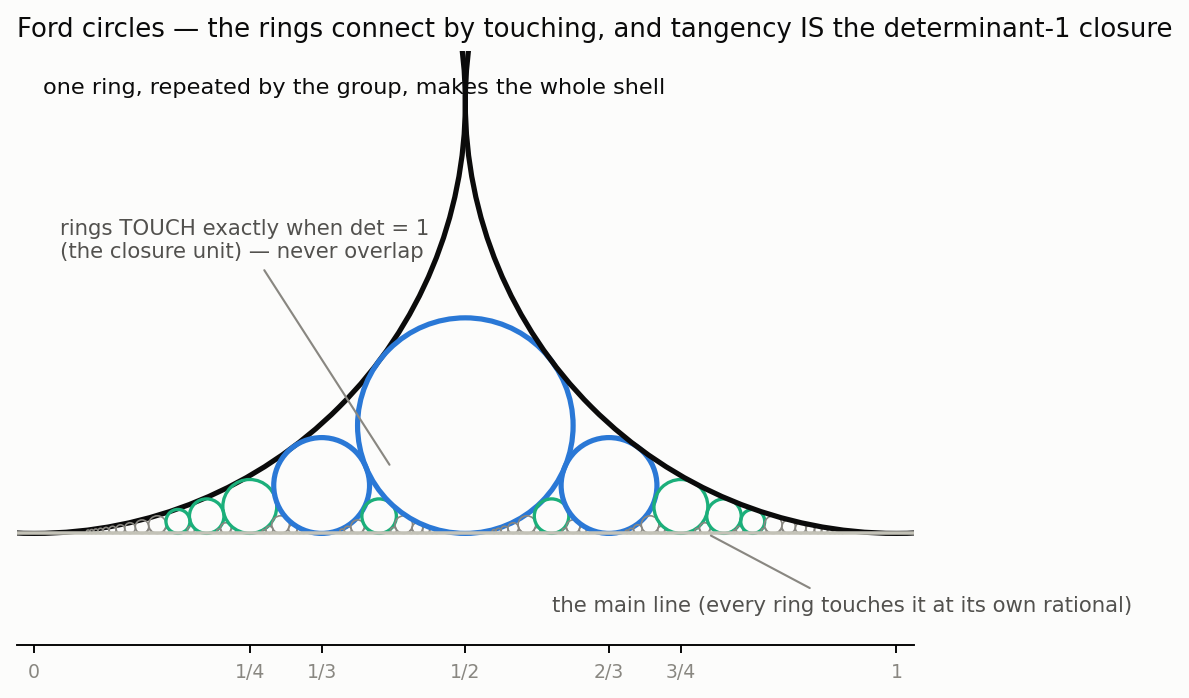
\includegraphics[width=0.85\textwidth]{ford_rings.png}
\caption{Ford circles: rings connect by touching, tangency occurring exactly at determinant 1; the
whole shell is one ring repeated by the modular group.}
\label{fig:ford}
\end{figure}

\begin{figure}[t]
\centering
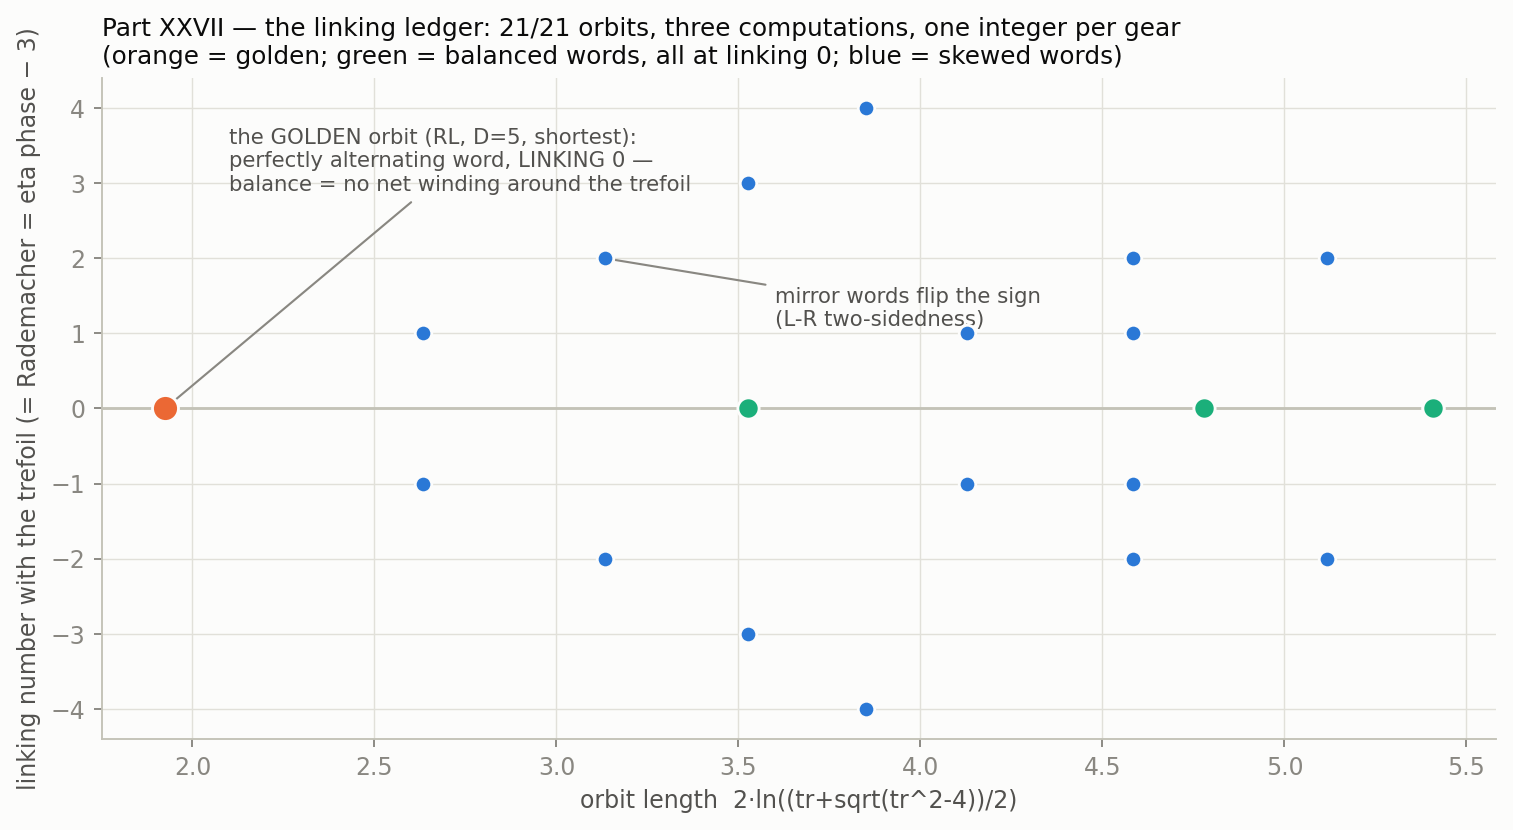
\includegraphics[width=0.75\textwidth]{linking_ledger.png}
\caption{The linking ledger: 21 orbits, three computations, one integer per gear; the golden orbit
and all balanced words at linking 0; mirror antisymmetry.}
\label{fig:linking}
\end{figure}

\begin{figure}[t]
\centering
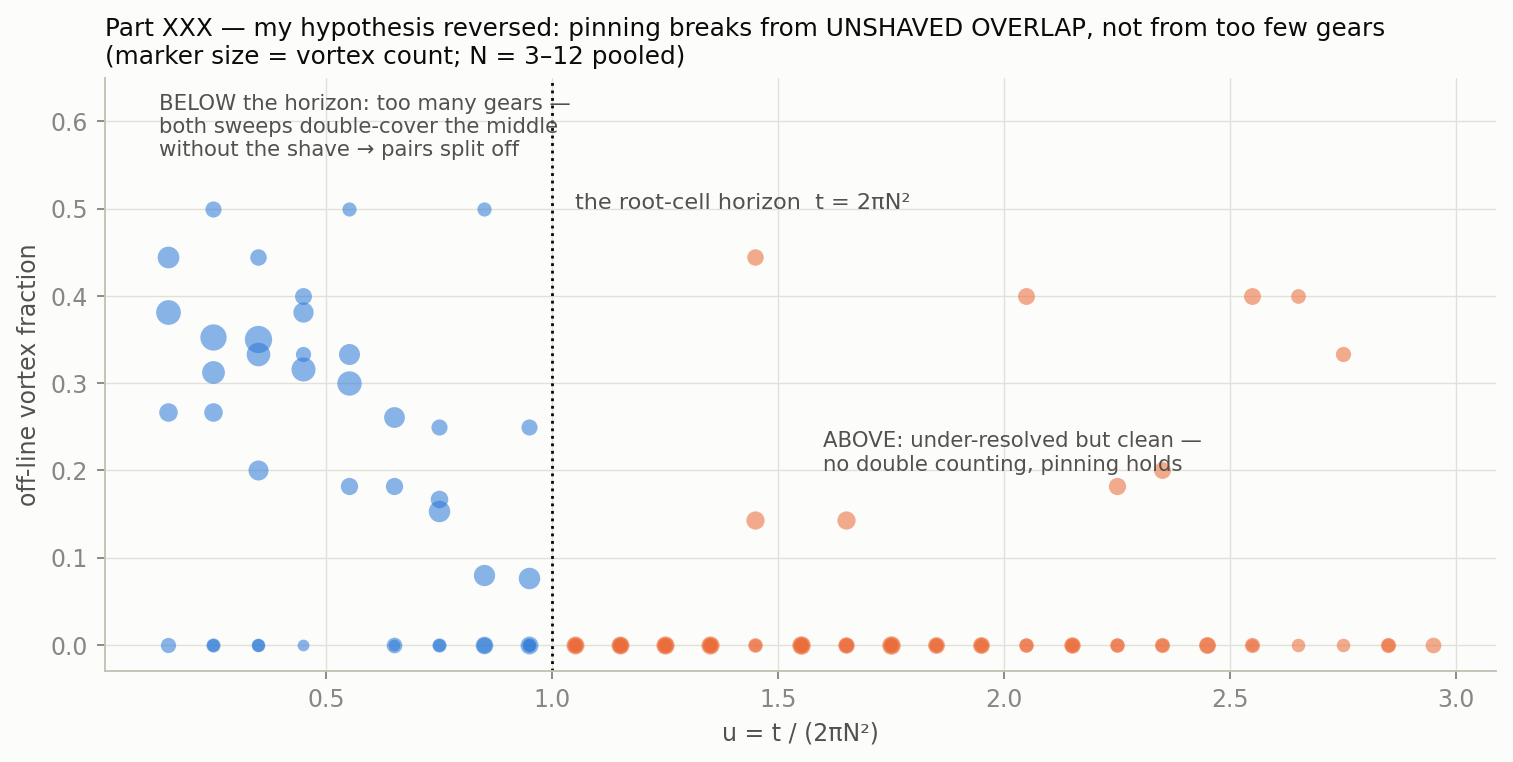
\includegraphics[width=0.8\textwidth]{melting.png}
\caption{The melting laboratory: off-line vortex fraction vs $u=t/(2\pi N^2)$. Defects concentrate
BELOW the root-cell horizon, where the two sweeps double-cover without the overlap subtraction ---
the shave is the pinning mechanism.}
\label{fig:melting}
\end{figure}

\section*{Methods and artifacts}
All computations were performed in-session with mpmath (zeta, Dirichlet $L$, Riemann--Siegel
functions; typically 15--25 digits), NumPy/SciPy (spectra, statistics, field solves), and PDB
structures from the RCSB. Scripts, figures, and intermediate data are archived alongside the
21-part laboratory log \texttt{FOLDING\_CRITICAL\_LINE.md} in the project repository; each figure in
this paper is reproduced by a named script (\texttt{pipeline.py}, \texttt{analysis.py},
\texttt{dbn\_lab.py}, \texttt{chi5\_lab.py}, \texttt{interleave.py}, \texttt{bk\_lab.py},
\texttt{ihara\_lab.py}, \texttt{meter\_lab.py}, \texttt{nb\_li\_lab.py}, \texttt{theta\_bridge.py},
\texttt{gear\_lab.py}, \texttt{xray\_fig.py}). Statistical conventions: Kolmogorov--Smirnov against
numerically integrated Wigner-surmise CDFs; nulls by degree-preserving edge swaps, circular shifts,
or color shuffles as stated; all $p$-values two-sided unless noted.

\section*{Acknowledgments}
The laboratories were designed and run in collaboration with Claude (Anthropic), which performed the
computations and drafted this manuscript from the session's laboratory log.

\begin{thebibliography}{20}\small
\bibitem{pelchat-theta} J.~Pelchat, \emph{Information-Theoretic Field Theory and the Resolution of
Multi-Body Gravitational Dynamics}, preprint (2025).
\bibitem{riemann} B.~Riemann, \emph{\"Uber die Anzahl der Primzahlen unter einer gegebenen
Gr\"osse}, Monatsber.\ Berlin.\ Akad.\ (1859).
\bibitem{montgomery} H.~Montgomery, The pair correlation of zeros of the zeta function,
Proc.\ Symp.\ Pure Math.\ 24 (1973).
\bibitem{odlyzko} A.~Odlyzko, On the distribution of spacings between zeros of the zeta function,
Math.\ Comp.\ 48 (1987).
\bibitem{berrykeating} M.~Berry and J.~Keating, $H=xp$ and the Riemann zeros, in
\emph{Supersymmetry and Trace Formulae} (1999); The Riemann zeros and eigenvalue asymptotics,
SIAM Review 41 (1999).
\bibitem{rodgerstao} B.~Rodgers and T.~Tao, The de Bruijn--Newman constant is non-negative,
Forum Math.\ Pi 8 (2020).
\bibitem{bostconnes} J.-B.~Bost and A.~Connes, Hecke algebras, type III factors and phase
transitions with spontaneous symmetry breaking in number theory, Selecta Math.\ 1 (1995).
\bibitem{julia} B.~Julia, Statistical theory of numbers, in \emph{Number Theory and Physics}
(1990).
\bibitem{landauer} R.~Landauer, Irreversibility and heat generation in the computing process,
IBM J.\ Res.\ Dev.\ 5 (1961).
\bibitem{bbls} L.~B\'aez-Duarte, M.~Balazard, B.~Landreau, E.~Saias, Notes sur la fonction
$\zeta$ de Riemann III, Adv.\ Math.\ 149 (2000).
\bibitem{li} X.-J.~Li, The positivity of a sequence of numbers and the Riemann Hypothesis,
J.\ Number Theory 65 (1997).
\bibitem{krzakala} F.~Krzakala et al., Spectral redemption in clustering sparse networks,
PNAS 110 (2013).
\bibitem{katzsarnak} N.~Katz and P.~Sarnak, \emph{Random Matrices, Frobenius Eigenvalues, and
Monodromy}, AMS (1999).
\bibitem{tate} J.~Tate, Fourier analysis in number fields and Hecke's zeta-functions, thesis
(1950), in \emph{Algebraic Number Theory} (1967).
\bibitem{connes} A.~Connes, Trace formula in noncommutative geometry and the zeros of the Riemann
zeta function, Selecta Math.\ 5 (1999).
\end{thebibliography}

\end{document}
